%\documentclass[prc,aps,preprint,floatfix]{revtex4}
\documentclass[aps,prc,twocolumn,floatfix]{revtex4}
%\usepackage[dvips]{graphicx}
%\usepackage{epsfig}
% \usepackage{pst-plot}
% \usepackage{bm}
\usepackage{appendix}
\usepackage{amsmath}
\usepackage{float}

% \usepackage{fullpage}
\usepackage{amsthm}
\usepackage{amsfonts}
\usepackage{graphicx}
% \usepackage[english]{babel}
% \usepackage[T1]{fontenc}
\usepackage{subfigure}
\usepackage{epstopdf}
% \usepackage[hyphens]{url}
%\usepackage{gensymb}
\usepackage{verbatim}
%\usepackage{slashed}
\usepackage{amssymb}
%\usepackage{amsfonts}
%\usepackage[toc,page]{appendix}


%% Define a new 'leo' style for the package that will use a smaller font.
\makeatletter
\def\url@leostyle{%
  \@ifundefined{selectfont}{\def\UrlFont{\sf}}{\def\UrlFont{\small\ttfamily}}}
\makeatother
%% Now actually use the newly defined style.
\urlstyle{leo}


%\usepackage[utf8]{inputenc}
%\usepackage{textcomp}
%\usepackage[T1]{fontenc}




\newcommand{\Fig}[1]{Figure~\ref{#1}}
\newcommand{\fig}[1]{figure~\ref{#1}}
\newcommand{\eq}[1]{equation~\ref{#1}}
\newcommand{\Eq}[1]{Equation~\ref{#1}}

% Shortcuts for including equations
\newcommand{\beq}{\begin{equation}}
\newcommand{\eeq}{\end{equation}}
\def\ivec{\textbf{i}}
\def\jvec{\textbf{j}}
\def\kvec{\textbf{k}}
\def\uvec{\textbf{u}}
\def\vvec{\textbf{v}}
\def\xvec{\textbf{x}}
\def\rvec{\textbf{r}}
\def\Rvec{\textbf{R}}
\def\cvec{\textbf{c}}
\def\S{\hat{S}}
\def\Svec{\hat{\textbf{S}}}
\def\H{\hat{H}}
\def\ro{\hat{\rho}}
\def\trace{\operatorname{Tr}}
\def\Lop{\hat{L}}
\def\etavec{\hat{\boldsymbol\eta}}
\def\X{\hat{X}}
\def\Y{\hat{Y}}
\def\etaop{\hat{\eta}}
\def\A{\hat{\textbf{A}}}
\def\B{\textbf{B}}
\def\aop{\hat{a}}
\def\aopd{\hat{a}^\dagger}
\def\bop{\hat{b}}
\def\bopd{\hat{b}^\dagger}
\def\alphavec{\boldsymbol\alpha}
\def\dvec{\textbf{d}}





% Document formatting
\setlength{\parindent}{0mm}
\setlength{\parskip}{1.5mm}

% Hyper refs
\usepackage[pdftex,colorlinks,breaklinks]{hyperref}
\usepackage{listings}
\usepackage{color}
\usepackage{textcomp}
\definecolor{listinggray}{gray}{0.9}
\definecolor{lbcolor}{rgb}{0.9,0.9,0.9}
\definecolor{pink}{RGB}{255, 119, 255}
\lstset{
	backgroundcolor=\color{lbcolor},
	tabsize=4,
	rulecolor=,
	language=c++,
        basicstyle=\scriptsize,
        upquote=true,
        aboveskip={1.5\baselineskip},
        columns=fixed,
        showstringspaces=false,
        extendedchars=true,
        breaklines=true,
        prebreak = \raisebox{0ex}[0ex][0ex]{\ensuremath{\hookleftarrow}},
        frame=single,
        showtabs=false,
        showspaces=false,
        showstringspaces=false,
        identifierstyle=\ttfamily,
        keywordstyle=\color[rgb]{0,0,1},
        commentstyle=\color[rgb]{0.133,0.545,0.133},
        stringstyle=\color[rgb]{0.627,0.126,0.941},
	title=\lstname
}

%\usepackage{multicol}  % used for the two-column index

\begin{document}
\title{Variational Monte Carlo for approximating ground states of Atoms and Molecules.}
\author{A. V. Solbr\aa}
\affiliation{Department of Physics, University of Oslo.} 

\date{\today}
\begin{abstract}
An Object Oriented code for performing Variational Monte Carlo (VMC) has been produced for measuring energies for Atoms and Molecules in order to search for the ground state energy and function. I run the code for He-, Be- and Ne-atoms, as well as $\text{H}_2$ and $\text{Be}_2$ molecules, using a simple slater determinant with a Jastrow factor ansatz. 
\end{abstract}

\maketitle

\section{Introduction}
\label{sec:introduction}
Variatinal Monte Carlo is a simple and useful way to approximate the ground state using some guess with a set of free parameters $\alphavec$. Since the Hamiltonian is hermitian we can expand our trial function $\psi_T(\rvec, \alphavec)$ in terms of the normalized eigenstates of the Hamiltonian as $\psi_T = \sum_i c_i \psi_i$, where for a normalized trial wave function, $\sum_i |c_i|^2  = 1$. The expectation value of the energy for the trial wave function is then $\langle \psi_T | \hat{H} | \psi_T \rangle = \sum_i c_i^2 E_i \ge E_0$, where $E_0$ is the energy of the ground state. We vary the parameters $\alphavec$ in order to find the lowest value of expectation value. In general our wave function is not normalized, and so our problem is to find \begin{equation}
\alphavec^* = \underset{\alphavec}{\operatorname{arg\,min}}\, {\langle \psi_T(\alphavec) | \hat{H} | \psi_T(\alphavec) \rangle \over \langle \psi_T(\alphavec) | \psi_T(\alphavec) \rangle }.
\end{equation}
And we then use $\psi_T(\rvec, \alphavec^*)$ as our approximation of the ground state, and we can use this state to calculate to an approximation to the ground state energy. 

\section{Monte Carlo integration and the Metropolis algorithm}
\label{sec:metro}
We want to calculate the integral 
\begin{equation}
 \langle E(\alphavec) \rangle = \frac{\int \psi^{\ast}_T(\rvec, \alphavec)\hat{H}(\rvec)\psi_T(\rvec, \alphavec) d\rvec} {\int\psi^{\ast}_T(\rvec, \alphavec)\psi_T(\rvec, \alphavec) d\rvec }
\end{equation}


The idea of Monte Carlo methods is to use the fact that
 \begin{equation}
  \int_V f(\rvec)\, d\rvec = \langle f \rangle V,
 \end{equation}
where $V$ is the domain of integration and $\langle f \rangle$ is the average value of $f$ in the domain. We then approximate the average as
\begin{equation}
 \langle f \rangle \approx {1 \over N} \sum_{i=1}^N f(x_i)
\end{equation}
where the $x_i$s are chosen by some rule. 

 Importance sampling is a method of choosing samples for the Monte Carlo method in a way such that the samples are as relevant as possible (e.g. in a way such that we avoid picking so many zero values in the above problem). Let's say that we want to find the integral of some function, $\int_a^b F(x)\, dx$ have some probability distribution $p(x)$, so that 
 \begin{equation}
  \int_a^b p(x) \, dx = 1.
 \end{equation}
We can then rewrite our integral as 
\begin{equation}
 I = \int_a^b F(x)\, dx = \int_a^b p(x) {F(x) \over p(x)}\, dx.
\end{equation}

Random numbers are generated for the uniform distribution on the unit interval $p(y)$ we need to perform a change of variables $y \rightarrow x$ through 
\begin{equation}
 y(x) = \int_a^x p(x')\,dx',
\end{equation}
If we can invert this equation, we can find $x(y)$. Now we can write our integral as
\begin{equation}
 I = \int_a^b F(x)\, dx = \int_a^b p(x) {F(x) \over p(x)}\, dx = \int_{\tilde{a}}^{\tilde{b}} {F(x(y)) \over p(x(y))}\, dy
\end{equation}
Note in particular the new integration limits. There is no definite way to chose the sampling function, but a nice trick is to choose a distribution which is a factor of the function we want to integrate, as this distribution will often look at least a bit like the integrand.

For expectation values of quantum observables there is a standard way of choosing the distribution. By noting that we can write our expectation value as 
\begin{align}
 \langle E(\alphavec) \rangle & = \frac{\int \psi^{\ast}_T(\rvec, \alphavec)\hat{H}(\rvec, \alphavec)\psi_T(\rvec, \alphavec) d\rvec} {\int\psi^{\ast}_T(\rvec, \alphavec)\psi_T(\rvec, \alphavec) d\rvec} \\
 & = \frac{\int \psi^{\ast}_T(\rvec, \alphavec){ \psi_T(\rvec, \alphavec) \over \psi_T(\rvec, \alphavec) }\hat{H}(\rvec, \alphavec)\psi_T(\rvec, \alphavec) d\rvec} {\int\psi^{\ast}_T(\rvec, \alphavec)\psi_T(\rvec, \alphavec) d\rvec} \\
 & = \frac{\int |\psi_T(\rvec, \alphavec)|^2{ 1 \over \psi_T(\rvec, \alphavec) }\hat{H}(\rvec, \alphavec)\psi_T(\rvec, \alphavec) d\rvec} {\int|\psi_T(\rvec, \alphavec)|^2 d\rvec}.
\end{align}
We now see that we can use the probability distribution 
\begin{align}
 p(\rvec, \alphavec) = { |\psi_T(\rvec, \alphavec)|^2 \over \int|\psi_T(\rvec, \alphavec)|^2 d\rvec }
\end{align}
If we now define the {\it local energy} as 
\begin{equation}
 E_L(\rvec, \alphavec) = {1 \over \psi_T(\rvec, \alphavec) }\hat{H}(\rvec, \alphavec)\psi_T(\rvec, \alphavec) 
\end{equation}
Then the expectation value of the energy can be written as
\begin{equation}
 \langle E \rangle = \int p(\rvec, \alphavec)E_L(\rvec, \alphavec) d\rvec.
\end{equation}
This all seems very nice, but we have so far overlooked the part about being able to invert the change of variables function. For our trial function, the probability density is invertible, and we must find some other way of drawing our samples. This is where the metropolis algorithm comes into the picture. 

The Metropolis algorithm is easy to state in its simplest form. Suppose we have found a first sample position $\Rvec$. We draw a candidate for a new step as $\Rvec' = \Rvec + \Delta \Rvec$, where $\Delta \Rvec$ has component drawn from a uniform distribution. We must perform two tests: 
\begin{enumerate}
 \item If 
 \begin{equation}
  {p(\Rvec') \over p(\Rvec)} > 1
 \end{equation}
 then the new step is accepted. 
 \item If not, the new step is accepted if
 \begin{equation}
  r \le {p(\Rvec') \over p(\Rvec)}
 \end{equation}
where $r$ is a uniform random variable on the unit interval. A nice advantage of this is that we do not ever need to compute the norm of the function as we are only computing ratios between probabilites. There is no absolute answer for what is the optimal acceptance rate of movements, but a good rule of thumb is to choose the distribution $\Delta \Rvec$ is drawn from such that we get an acceptance rate of 50\%. 
\end{enumerate}
\subsection{Importance sampling in the Metropolis algorithm}
 We want to keep the correlation between the Monte Carlo measurement low. An obvious way to do this would be to simply increase the step size, so that the wave function looks entirely different from one step to the next. The problem with this is that the acceptance rate would fall and we would keep selecting the same point over and over, which would give a high variance! This is where the acceptance rate ``rule of thumb'' of 0.5 comes from, but the optimal interval varies a lot from case to case.
 
 If we proposed our new steps in a better way, we could perhaps still improve the efficency of the step length versus acceptance rate. One way to do this is to modify our symmetrical selection rule such that the samples move towards areas of the state-space where the distribution is large. One such procedure is the Fokker-Planck formalism where the walkers are moved according to the gradient of the distribution. The formalism ``pushes'' the samples in a ``disireable'' direction. The idea is to propose moves similarly to an isotropic diffusion process with a drift. A new position $r_\text{new}$ is calculated from the old one, $r_\text{old}$ as
 \begin{equation}
  r_\text{new} = r_\text{old} + \chi + DF(r_\text{old}) \delta t.
 \end{equation}
Here, $\chi$ is a Gaussion randum number with mean 0 and $\sigma = \sqrt{2D\delta t}$. It accounts for the drift. $F$ is a drift velocity dependent on the position of the samples and is derived from the quantum mechanical wave function $\psi$. The constant $D$, being the diffusion constant of $\chi$, also adjusts the size of the drift. $\delta t$ is a time step parameter whose presence will be investigated. 

What is the optimal choice for the drift term? From statistical mechanics we know that a simple isotropic drift diffusion process obeys a Fokker-Planck equation of the form:
\begin{equation}
 {\partial f \over \partial t} = \sum_i D {\partial \over \partial x_i} \left( {\partial \over \partial x_i} - F_i(F)\right) f,
\end{equation}
where $f$ is the continuous distribution of samples. It can be shown that the drift velocity has to be chosen as follows: 
\begin{equation}
 F = {1 \over f} \nabla f,
\end{equation}
or in our case, where $f = |\psi|^2$, 
\begin{equation}
 F = 2{1\over \psi}\nabla \psi, 
\end{equation}
From our previous calculations, we note that 
\begin{equation}
 {\partial \over \partial x_1}\psi = \left( - {\alpha x_1 \over r_1} + {x_1-x_2 \over 2r_{12}(\beta r_{12} + 1)^2} \right) \psi
\end{equation}
which lets us implement a closed form of the gradient.

With this new step selection rule, according to the Metropolis algorithm the requirement for accepting a step is also modified. The previus one, 
\begin{equation}
P(r_\text{new}, r_\text{old}) = \min(1,q(r_\text{new}, r_\text{old}))
\end{equation}
with 
\begin{equation}
 q(r_\text{new}, r_\text{old}) = |\psi(r_\text{new})|^2/ |\psi(r_\text{old})|^2 |\psi(r_\text{new})|^2/ |\psi(r_\text{old})|^2
\end{equation}
is now replaced with 
\begin{equation}
 q(r_\text{new}, r_\text{old}) = {G(r_\text{old}, r_\text{new},\Delta t)|\psi(r_\text{new})|^2 \over G(r_\text{new},r_\text{old}, \Delta t) |\psi(r_\text{old})|^2 }
\end{equation}
where $G$ is the Green's function
\begin{widetext}
 \begin{equation}
  G(r_\text{new},r_\text{old}, \Delta t) = {1 \over (4\pi D \Delta t)^{3N/2}}\exp\big(-(\rvec_\text{new} - \rvec_\text{old} - D\Delta t F(r_\text{old}))^2/4D\Delta t\big)
 \end{equation}
 \end{widetext}

 This produces the same results as our previous algorihm, however, by choosing a small value for $\Delta t$ we can get a much higher acceptance rate, which means we will get a smaller error, as shown in figure \ref{fig:1}
 
  \begin{figure}
\centering
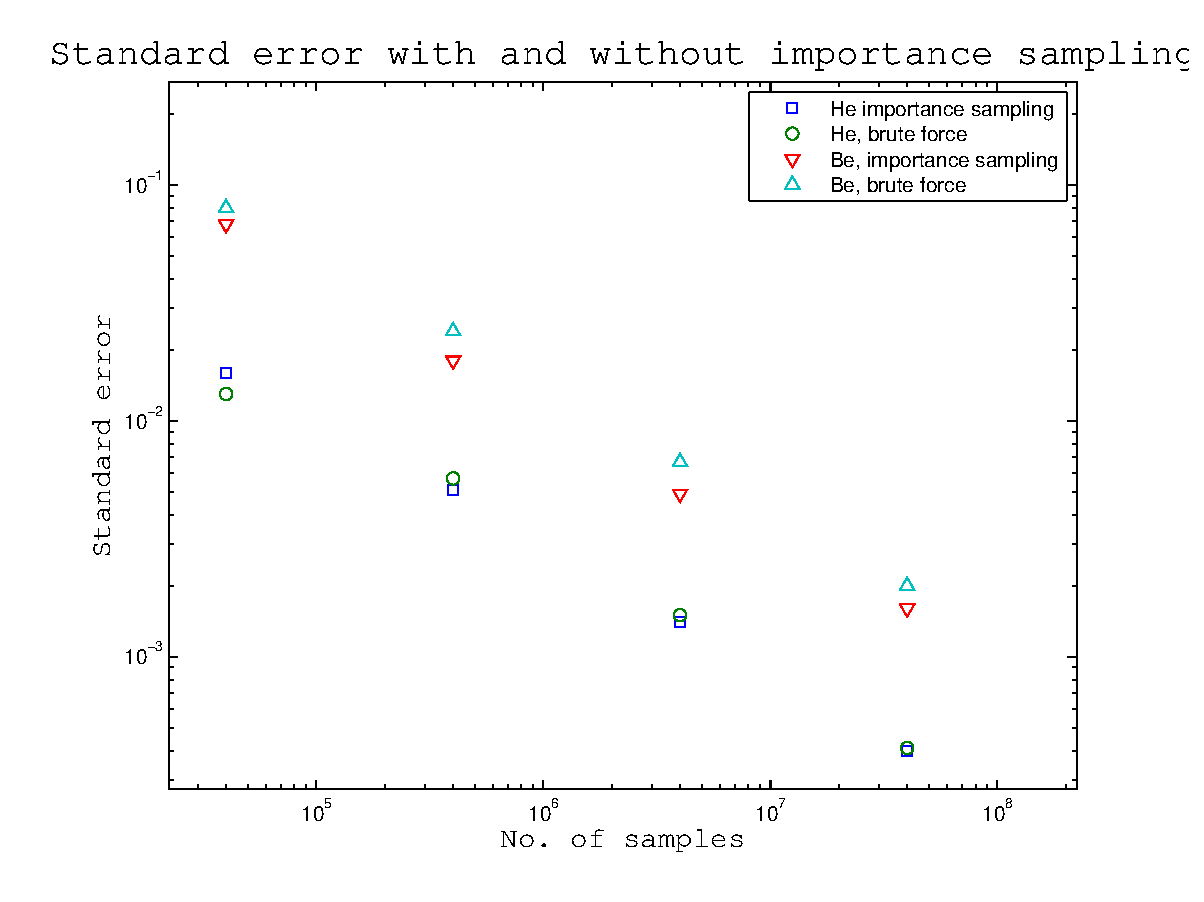
\includegraphics[width=9cm]{figures/errors.eps}
\caption{\label{fig:1} The figure shows the standard errors for He and Be, with and without importance sampling. The standard errors are calculated as detailed in section \ref{sec:block}.}
\end{figure}
 
\section{Hamiltonian and ansatz for the wave function}
\label{sec:ansatz}
 The Helium atom is the simplest possible system besindes the hydrogen atom. If we let $\rvec_1$ describe the position of the the first electron relative to the nucleus, and $\rvec_2$ likewise describe the position of the second electron, the in potential energy is from the interactions between the electrons and the nucleus can be described as
 \begin{equation}
  V_{\rm nuc}(\rvec_1, \rvec_2) = -{Z \over 4 \pi \epsilon_0}\left( {1 \over r_1} + {1 \over r_2} \right),
 \end{equation}
where $r_1$ is the length of $\rvec_1$ and $Z$ is the number of protons in the nucleus, e.g. 2 for Helium. It is preferrable to work with dimensionless units, so let us from this point on work in distance units of $\hat{r} = 4\pi \epsilon_0 r$. The hats will be cumbersome, so we will simply use $r$. In dimensionless units, the nucleus potential is written as 
\begin{equation}
 V_{\rm nuc}(\rvec_1, \rvec_2) = -Z\left( {1 \over r_1} + {1 \over r_2} \right).
\end{equation}
We should also include the interactions between the particles, making the full potential 
\begin{equation}
 V = -{Z \over r_1} - {Z \over r_2} + {1 \over r_{12}}
\end{equation}
yielding the total Hamiltonian 
\begin{equation}
 H(\rvec_1, \rvec_2) = -{\nabla^2_1 \over 2} -{\nabla^2_2 \over 2}-{Z \over r_1} - {Z \over r_2} + {1 \over r_{12}}
\end{equation}
For an atom with $n$ particles, the general Hamiltonian is
\begin{equation}
 H(\{ \rvec_i \}) = \sum_{i=1}^n \left( {-\nabla_i^2 \over 2} - {Z \over r_i} + \sum_{j=i+1}^n {1 \over r_{ij}} \right)
\end{equation}

In this project we will assume the wavefunction to be comprised of hydrogen-like orbitals, as well as a correlation term in the form of a Jastrow factor, i.e. we let our ansatz be 
\begin{equation}
 \Psi_T(\alpha, \beta, \{\rvec\}) = \Psi_S(\alpha, \{\rvec\} ) \Psi_C(\beta,\{\rvec\})
\end{equation}
where 
\begin{align}
 \Psi_S(\alpha, \rvec_1, \rvec_2, \ldots, \rvec_n) = \begin{vmatrix}
  \phi_1(\rvec_1) & \phi_2(\rvec_1) & \ldots & \phi_4(\rvec_1)\\
  \phi_1(\rvec_2) &  & & \vdots \\
  \vdots &  & \ddots & \\
  \phi_1(\rvec_n) & \ldots  &  & \phi_n(\rvec_n)
\end{vmatrix}
\end{align}
is the slater-determinant of the lowest orbitals with $\alpha$ as an effective charge, i.e.
\begin{align}
 \phi_{1s}(\rvec) & = \exp(-\alpha r), \\
 \phi_{2s}(\rvec) & = (1-\alpha r/2)\exp(-\alpha r/2), \\
 \phi_{2p}(\rvec) & = \alpha \rvec \exp(-\alpha r/2)
\end{align}
where we use solid harmonics for the different $m_l$ states of the $2p$ orbital. Note that each function is used twice to account for the different spin orientations. The correlation term is 
\begin{equation}
 \Psi_C(\beta, \{ \rvec_i \}) = \prod_{i<j} \exp\left({a_{ij} r_{ij} \over 1 + \beta r_{ij}} \right),
\end{equation}
where $a_{ij} = 1/2$ if particles $i$ and $j$ have opposite spin, and $a_{ij} = 1/4$ otherwise. 


\subsection{Efficient computation of the wave function properties}
One complication is that the Slater Determinant is very expensive to compute for larger systems (the computation of a determinant of an $N \times N$ matrix goes as $O(N^3)$ in the leading term). It is worthwhile to find better methods of computing this determinant. 

The first thing we do is to note that, as shown by for example \cite{moskowitz81}, that for the variational energy we can approximate the determinant as 
\begin{equation}
 \phi(\rvec_1, \rvec_2, \ldots, \rvec_n) \propto \operatorname{Det}\uparrow \operatorname{Det}\downarrow
\end{equation}
where we put the first half of the electrons in the first determinant, and the other half in the second determinant. This is valid for spin independent hamiltonians. Using this we can write our wave function as $\psi_T (\rvec) = D_\uparrow D_\downarrow \psi_C$. This is already a significant speedup! However, we will now look into a far more efficient way of calculating ratios of wavefunctions, like those we will need in the metropolis algorithm.
\subsubsection{Closed expressions for local energy}
When implementing the closed form expression for the energy, we calculate
\begin{equation}
 {1 \over \psi_T} \hat{H} \psi_T
\end{equation}
where the challenge is calculating the $\nabla^2_1\psi$ term. Let us see if we are able to calculate this term in our more general case. Our wavefunction can be factorized as 
\begin{equation}
 \psi_T(\{ \rvec_i \}) = \psi_S(\{ \rvec_i \})\psi_C(\{\rvec_i \})
\end{equation}
where $\psi_S$ is the Slater Determinant, and $\psi_C$ contains the jastrow factor. In this way, we can write the laplacian as 
\begin{equation}
 \nabla_i^2 \psi_T = \psi_C \nabla_i^2 \psi_S + 2 \nabla_i \psi_S \cdot \nabla_i \psi_S + \psi_S \nabla_i^2 \psi_C^2.
\end{equation}
The expressions for the gradients and laplacians are given in Appendix \ref{sec:gradlap}.

\subsection{Hamiltonian and ansatz for molecules}
The $\text{H}_2$ molecule consists of two protons and two electrons with a ground state energy.
$E = -1.175$ a.u. and the equilibrium distance between the two
hydrogen atoms of $r_0 = 1.40$ Bohr radii.

We define our systems using the following variables. Origo is chosen to be halfway
between the two protons. The distance from proton 1 is defined as $\Rvec/2$ whereas
proton 2 has a distance $-\Rvec/2$. Calculations are performed for fixed distances $\Rvec$ between the two protons.

Electron 1 has a distance $r_1$ from the chose origo, while electron 2 has a distance $r_2$. The kinetic energy operator then becomes 
\begin{equation}
 -{\nabla^2_1 \over 2} - {\nabla^2_2 \over 2}.
\end{equation}
The distance between the two electrons is $r_{12} = |\rvec_1 - \rvec_2|$. The repulsion between the two electrons results in a potential energy term given by 
\begin{equation}
 +{1\over r_{12}}.
\end{equation}
In a similar way we obtain a repulsive contribution from the interaction between the two protons given by 
\begin{equation}
 + {1\over |\Rvec|}
\end{equation}
For general elemental gasses the term becomes ${Z^2/ |\Rvec|}$. 

To obtain the final potential energy we need to include the attraction the attraction the electrons feel from the protons. To model this, we need to define the distance between the electrons and the two protons. If we model this along a chosen z-axis with electron 1 placed at a distance $\rvec_1$ from a chosen origin, one proton at $-\Rvec/2$ and the other at $\Rvec/2$, the distance from proton 1 to electron 1 becomes
\begin{equation}
 \rvec_{1p1} = \rvec_1 + \Rvec/2
\end{equation}
and 
\begin{equation}
\rvec_{1p2} = \rvec_1 - \Rvec/2
\end{equation}
from proton 2. 

Similarly, for electron 2 we obtain
\begin{equation}
 \rvec_{2p1} = \rvec_2 + \Rvec/2
\end{equation}
and 
\begin{equation}
 \rvec_{2p2} = \rvec_2 - \Rvec/2
\end{equation}
These four distances define the attractive contributions to the potential energy, 
$$
-{1\over r_{1p1}} - {1 \over r_{1p2}} - {1\over r_{2p1}} - {1 \over r_{2p2}}.
$$
And the complete hamiltonian becomes 
\begin{equation}
 \hat{H} =  -{\nabla^2_1 \over 2} - {\nabla^2_2 \over 2} -{1\over r_{1p1}} - {1 \over r_{1p2}} - {1\over r_{2p1}} - {1 \over r_{2p2}} + {1\over r_{12}} + {1\over |\Rvec|}
\end{equation}


For $\text{H}_2$, we will use a trial wave function of the form 
\begin{equation}
 \psi_T(\rvec_1, \rvec_2, \Rvec) = \psi(\rvec_1, \Rvec)\psi(\rvec_2,\Rvec)\exp\left( {r_{12} \over 2(1+\beta r_{12})} \right).
\end{equation}
with the following trial wave function 
\begin{equation}
 \psi(\rvec_1, \Rvec) = (\exp(-\alpha r_{1p1})  + \exp(-\alpha r_{1p2})),
\end{equation}
for electron 1, and 
\begin{equation}
 \psi(\rvec_2, \Rvec) = (\exp(-\alpha r_{2p1}) + \exp(-\alpha r_{2p2}))
\end{equation}
for electron 2. 

The question arises of how to construct the higher orbitals. One approach that ensures as many electrons in the bottom states as possible, is to let the next wavefunctions be 
\begin{equation}
 \psi(\rvec_1, \Rvec) = (\exp(-\alpha r_{1p1})  - \exp(-\alpha r_{1p2})),
\end{equation}
for electron 1, and 
\begin{equation}
 \psi(\rvec_2, \Rvec) = (\exp(-\alpha r_{2p1}) - \exp(-\alpha r_{2p2}))
\end{equation}
for electron 2. We then use sums and differences of the $|2,0,0 \rangle$ states for the four next electrons, and so on. These first 8 wavefunctions allows us to simulate the beryllium molecule as well. 


\section{Minimization algorithm for the energy}
\label{sec:minimize}

Using brute force methods as described earlier is well and good for making energy plots such as in figures \ref{fig:1} and \ref{fig:3}. However, when we want to do a large scale simulation in order to calculate the energy with an as small error as possible, we would rather only use a large number of samples for the minimal energy. We need some method of finding the minimal energy. We will focus on {\it gradient methods}, iterative methods given by 
 \begin{equation}
  \alphavec_{k+1} = \alphavec_k + c_k\dvec_k
 \end{equation}
where $\nabla E(\alphavec)^T \dvec_k < 0$, i.e. we move in directions where the gradient is negative. There are many different wany to chose the direction $\dvec_k$: 
\begin{itemize}
 \item If we choose $\dvec_k = -\nabla E(\alphavec_k)$ we get the {\it steepest descent method},
 \begin{equation}
  \alphavec_{k+1} = \alphavec_k - c_k\nabla E(\alphavec_k)
 \end{equation}
 
 \item The steepest descent method can be thought of as a first order approximation to the gradient of $E$. A second order approximation gives us Newtons method, 
 \begin{equation}
   \alphavec_{k+1} = \alphavec_k - c_k(\nabla^2 E(\alphavec_k))^{-1} \nabla E(\alphavec_k)
 \end{equation}
 where $\nabla^2$ here means the hessian matrix, not the laplacian.

 \item The conjugate gradient method chooses new direction orthogonal to the previous one. It can be sumarized in three steps. First you calculate the residual, 
 \begin{equation}
  \rvec_k = - \nabla E(\alphavec)
 \end{equation}
 then you find the new direction by the gram-schmidt process as 
 \begin{equation}
  \dvec_{k} = \rvec_k - \sum_{i < k} {\dvec_i^T \nabla^2 E(\alphavec) \rvec_k \over \dvec_i^T \nabla^2 E(\alphavec) \dvec_i}\dvec_i
 \end{equation}
 and then finally we find the new values as
 \begin{equation}
  \alphavec_{k+1} = \alphavec_k + c_k\dvec_k
 \end{equation}
 
\item Broyden's method is a quasi-Newton method, that uses updates the position as 
\begin{equation}
 \alphavec_{k+1} = \alphavec_k - B_k\nabla E(\alphavec_k)
\end{equation}
for some matrix $B_k$. The next matrix is then found as 
\begin{equation}
 B_{k+1} = B_k + {1 \over s_k^T s_k}(y_k - B_k s_k)s_k^T
\end{equation}
where $s_k = \alphavec_{k+1} - \alphavec_k$ and $y_k = E(\alphavec_{k+1}) - E(\alphavec_k)$. This can be thought of as a multi-dimensional secant method, and it can be shown that $B_k$ approximates the hessian well, given that the initial expression is good. 


\end{itemize}
It turns out that all of these methods are quite dissappointing in our case, much because there are large uncertainties in our expressions for the gradient. We will implement an adaptive method, where the step direction is simply along the signs of the gradient, and the step rule is to half the step each time the derivative changes sign, and multiply the step with 1.1 when it does not. Such a minimization search is illustrated in figures \ref{fig:addap1} and \ref{fig:addap2}.
 
  \begin{figure}
\centering
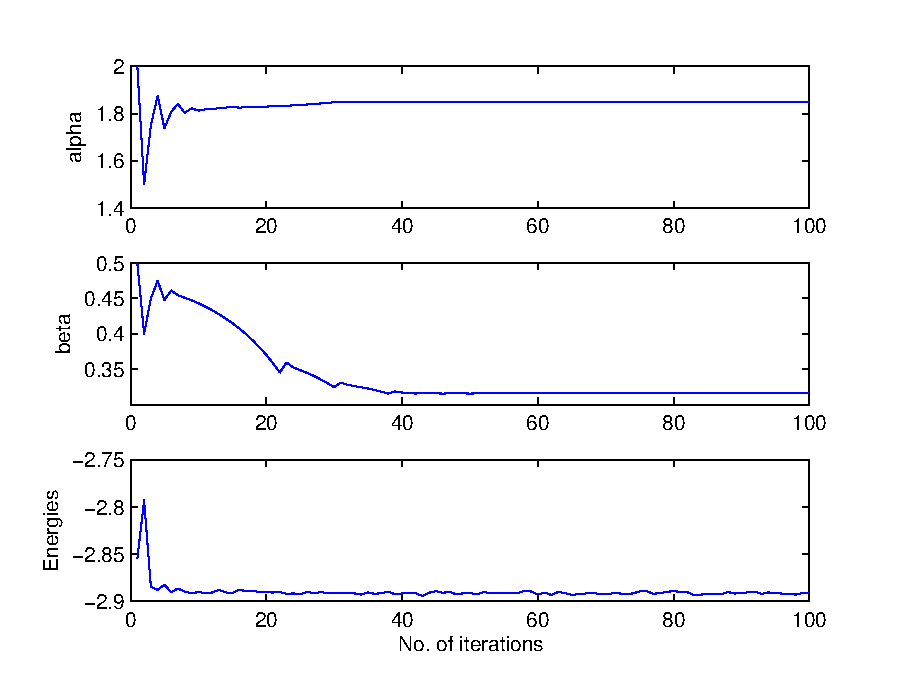
\includegraphics[width=7cm]{figures/addaptiveplot1.eps}
\caption{\label{fig:addap1} The figure shows the evolution of the parameter values of $\alpha$ and $\beta$ using the addaptive method detailed in section \ref{sec:minimize}}
\end{figure}

 \begin{figure}
\centering
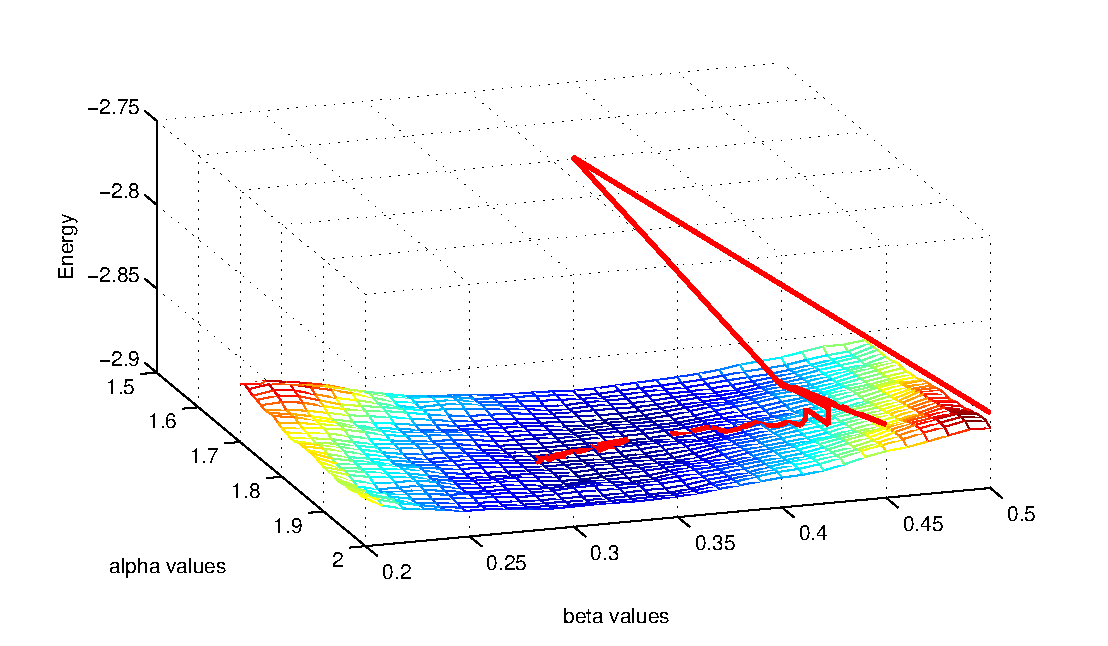
\includegraphics[width=7cm]{figures/addaptiveplot2.eps}
\caption{in the energy space using the addaptive method detailed in section \ref{sec:minimize}}
\end{figure}
 
 \subsection{Expressions for the gradient}
 One can show the following expressions
 \begin{equation}
  {\partial  \over \partial \alpha_i}\langle E \rangle = 2\left(  \left\langle {1 \over \psi(\alphavec)} {\partial \psi(\alphavec) \over \partial \alpha_i}  E_L(\alphavec) \right\rangle - \left\langle E_L(\alphavec) \right\rangle \left\langle {1 \over \psi(\alphavec)} {\partial \psi(\alphavec) \over \partial \alpha_i} \right\rangle \right)
 \end{equation}
As for our spesific case, 
\begin{equation}
 {1\over \psi}{\partial \psi \over \partial \alpha} = {1\over D}{\partial D \over \partial \alpha} = \sum_{i,j} {\partial \phi_{ij} \over \partial \alpha} D_{ji}^{-1}
\end{equation}
and 
\begin{equation}
 {1 \over \psi} {\partial \psi \over \partial \beta} = {1 \over \psi_C} {\partial \psi_C \over \partial \beta} = \sum_{i=1}^N \sum_{j=i+1}^N a_{ij}r_{ij}^2/(1+\beta r_{ij})^2
 \end{equation}
These expressions will make the gradient fast and more reliable to calculate, as opposed to numerical derivatives. 

\section{Statistical analysis using Blocking}
\label{sec:block}
 We want an estimate on how good our Monte Carlo result is. If we find an average of $N$ uncorrolated measurements, then the standard deviation of the mean you found is given by the well known result 
 \begin{equation}
  \sigma_N = {1 \over \sqrt{N}}\sigma
 \end{equation}
where $\sigma$ is the standard deviation in the individual draws. But our draws using the metropolis algorithm are not uncorrolated. Far from it! Each step is absolutely dependent on the position of the previous step. In effect, this means that the above formula will give too nice an error estimate. 

One step is affected by the previous step. But what about the step before that, or 10, 100 1000, 10 000 steps before that? The idea that chunks of steps far appart will be mostly uncorrelated forms the idea behind the blocking method. What we do is simply to collect blocks of $m$ samples, find the average of these, and use the standard deviations in them to calculate $\sigma_N$ as 
\begin{equation}
 \sigma_N = {1 \over \sqrt{m}} \sigma_m
\end{equation}
where $\sigma_m$ is the standard deviation of the averages in the blocks. The effectiveness of this method is shown in \cite{flyvberg89}, we here simply note that if the samples were uncorrolated to begin with, this procedure will give the same result as calculating the error normally, regardless of $m$. 
 
Figure \ref{fig:block} shows an example of a blocking result (The data is taken from a Neon run which is detailed in section \ref{sec:res}). The error is read off as the maximum of the curve.

  \begin{figure}
\centering
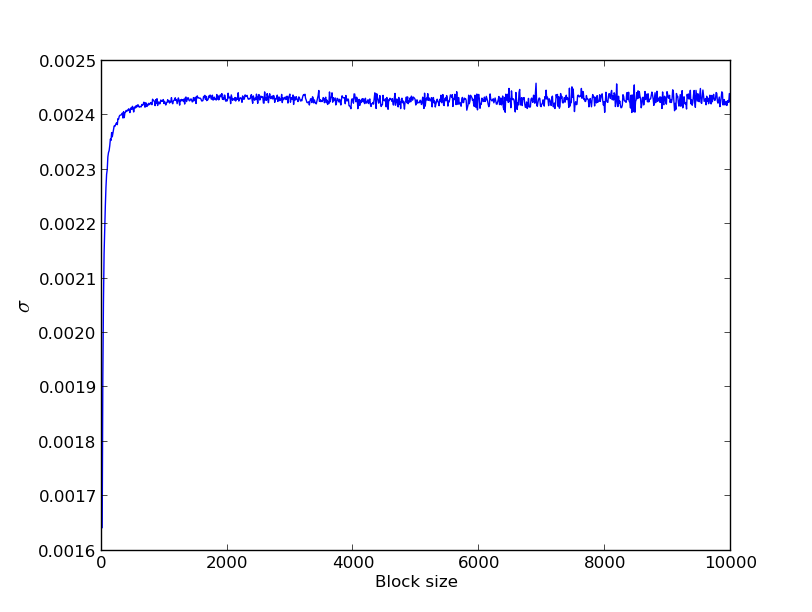
\includegraphics[width=7cm]{figures/blockingex.png}
\caption{\label{fig:block} The figure shows a typical example of a blocking analysis result.}
\end{figure}

\subsection{Error as a function of the Metropolis time step}
The parameter $\Delta t$ in the Metropolis algorithm sets the average trial step length. A too large step will give a small acceptance probability, while a too small step will move the walker an insignifigant amount. Both of these extremes lead to highly correlated data, and as such choosing the right $\Delta t$ is important to obtain good results. Figure \ref{fig:blockdt} shows the result of an experimental search for the right $\Delta t$. 

  \begin{figure}
\centering
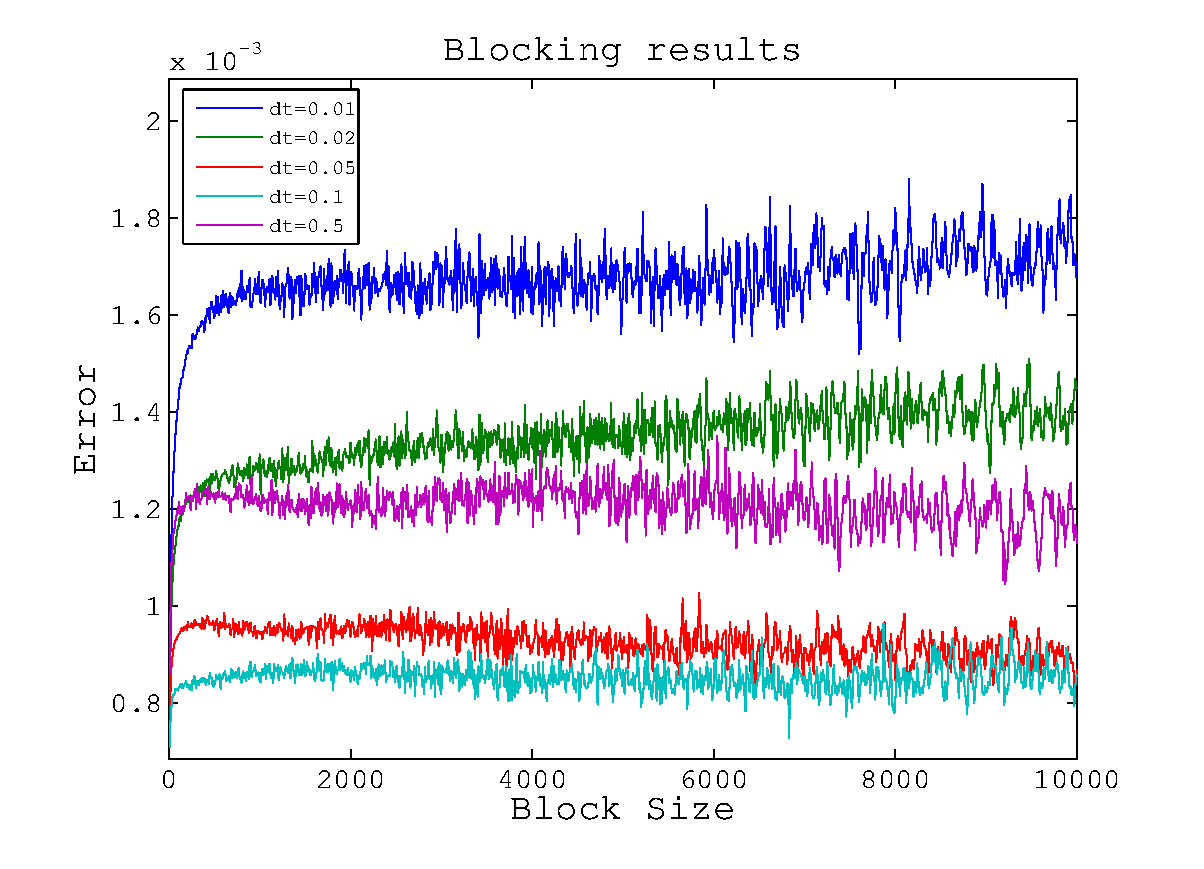
\includegraphics[width=7cm]{figures/blockingdt.eps}
\caption{\label{fig:blockdt} The figure shows the blocking results for many different $\Delta t$s. The results are obtained from runs of the Helium atom, using $10^6$ Monte Carlo cycles.}
\end{figure}

\section{VMC calculations for $\text{He}$, $\text{Be}$, $\text{Ne}$, $\text{H}_2$ and $\text{Be}_2$}
\label{sec:res}
The adaptive method described in section \ref{sec:minimize} was run for the different systems, after which a large scale Monte Carlo Simulation was run to calculate the optimal energies. The results for atoms are summarized in table \ref{tab:3}, and the results for molecules are summarized in table \ref{tab:4}.
\begin{table}
\centering
 \begin{tabular}{|ccccccccc|}
  \hline
  Atom & $\alpha$ & $\beta$ & $E_\text{VMC}$ & $E_0$ & $N$ & $\sigma_\text{std}$ & $\langle r_{ij} \rangle$ & $\tilde{\epsilon}$ \\
  \hline 
  He & 1.84 & 0.34 & -2.8908 & -2.9037 & $10^8$ & 4e-4 & 1.363 & 4.44e-3\\
  He & 2.0 & 0.175 & -2.84267 & -2.9037 & $4\times 10^7$ & 8e-4 & 1.284 & ... \\
  He & 2.0 & - & -2.740 & -2.9037 & $4\times 10^7$ & 1e-3 & 1.085 & ...  \\
  He & 1.69 & - & -2.8426 & -2.9037 & $4\times 10^7$ & 9e-4 & 1.28 & ... \\
  Be & 3.88 & 0.12 & -14.4827 & -14.6664 & $10^8$ & 5e-4 & 1.31 &  1.25e-2\\
  Be & 4.0 & 0.087 & -14.4743 & -14.6664 & $4\times 10^7$ & 2e-3 & 2.25 & ...  \\
  Be & 4.0 & - & -13.696 & -14.6664 & $4\times 10^7$ & 3e-3 & 1.48 & ...  \\
  Be & 3.37 & - & -14.213 & -14.6664 & $4\times 10^7$ & 3e-3 & 1.76 & ...  \\
  Ne & 10.33 & 0.073 & -127.607 & -128.884 & $10^8$ & 3e-3 & 1.18 & 1.00e-2\\
  Ne & 10 & 0.104 & -127.63 & -128.884 & $4\times 10^6$ & 2e-2  & 1.18 & ...\\
  Ne & 10 & - & -112.20 & -128.884 & $4\times 10^6$ & 6e-2 & 0.68 & ...\\
  Ne & 7.81 & - & -121.88 & -128.884 & $4\times 10^6$ & 9e-2 & 0.87 & ...\\
  \hline
 \end{tabular}

 \caption{The table shows a summary of VMC results for He, Be and Ne. $\alpha$ and $\beta$ are the variational parameters, $E$ is the optimal energy attained, $E_0$ is the experimental value of the energy, $N$ is the number of monte carlo cycles,   $\sigma_{\text{std}}$ is the standard error calculated as explained in section \ref{sec:block}, $\langle r_{ij} \rangle$ is the average electron separation and $\tilde{\epsilon}$ is the relative error of the VMC result compared to the experimental value.}
 \label{tab:3}
 \end{table}

\begin{table}
\centering
 \begin{tabular}{|cccccccccc|}
  \hline
  Molecule & $R$ & $\alpha$ & $\beta$ & $E_{\text{VMC}}$& $E_0$ & $N$ & $\sigma_\text{std}$ & $\langle r_{ij} \rangle$ & $\tilde{\epsilon}$ \\
  \hline 
  $\text{H}_2$ & 1.4 & 1.29 & 0.39 & -1.1584 & -1.175 & $10^7$ & 4e-4 & 2.17 & 1.41e-2\\
  $\text{Be}_2$ & 4.63 & 3.65 & 0.55 & -28.6927 & -29.3385 & $10^7$ & 3e-3 & 3.75 & 2.20e-2 \\
  \hline
 \end{tabular}

 \caption{summary of VMC results for $\text{He}_2$ and $\text{Be}_2$. $\alpha$ and $\beta$ are the variational parameters, $E$ is the optimal energy attained, $E_0$ is the experimental value of the energy, $N$ is the number of monte carlo cycles,   $\sigma_{\text{std}}$ is the standard error calculated as explained in section \ref{sec:block}, $\langle r_{ij} \rangle$ is the average electron separation and $\tilde{\epsilon}$ is the relative error of the VMC result compared to the experimental value.}
 \label{tab:4}
\end{table}



\subsection{One-body densities}
Using the optimal parameters detailed in the previous section, we can produce the one-body densities of the different systems. This is done by noting that the Metropolis algorithm creates the distribution defined by the wave function. So we simply store that walker positions for a large number of Monte Carlo cycles, and make histograms of the walker positions.

We note that even though minimization over $\alpha$ only, without including the Jastrow factor, gives good approximations to the energies, the one-body densities are quite different. When only minimizing over $\beta$ however, we get densities very close to the complete minimization result. This hints that the correlation term is vital for obtaining good approximations to the ground state. This is especially evident in the cases for Beryllium and Neon.

\begin{figure}[ht]
\subfigure[radial distribution]{
	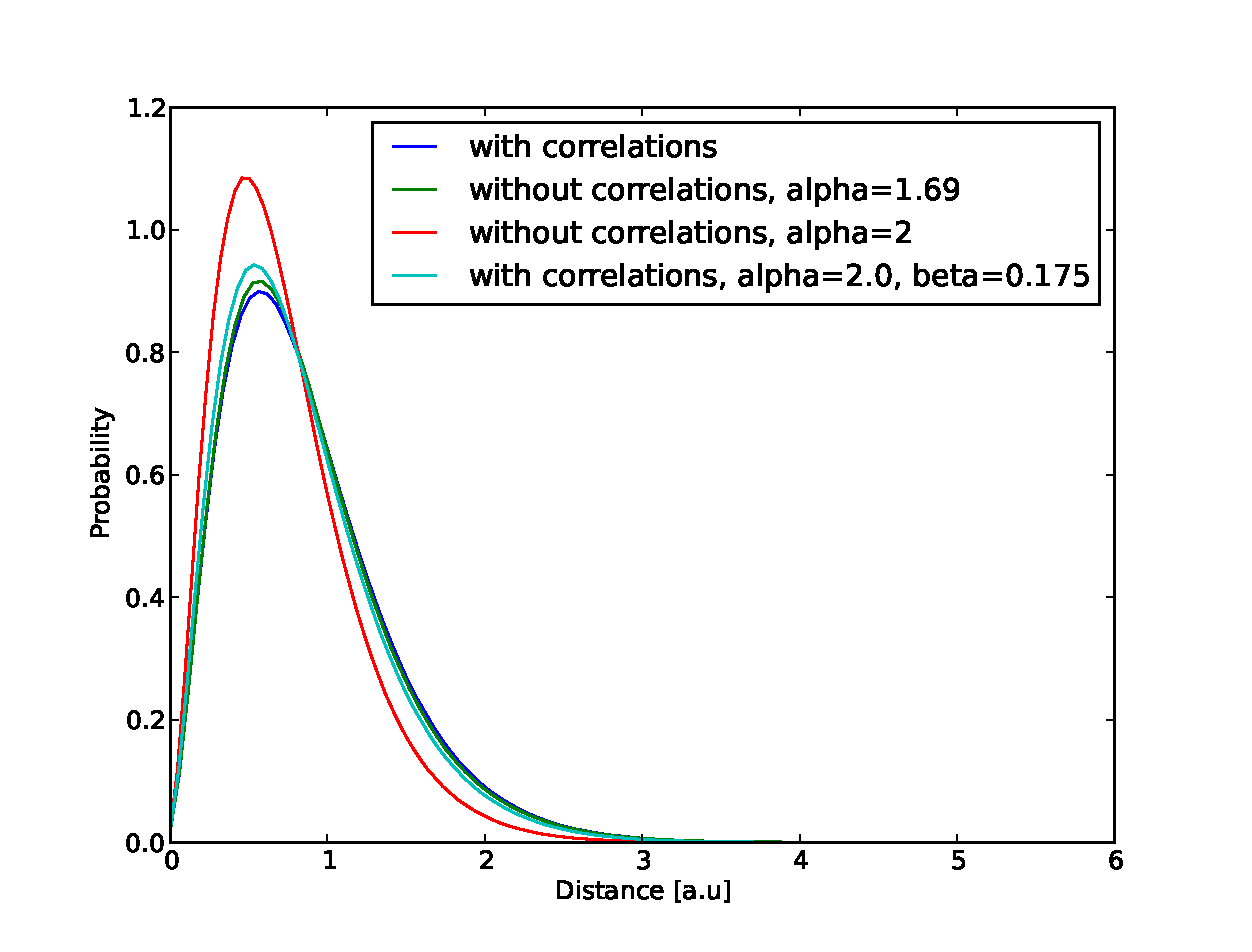
\includegraphics[width=6cm]{figures/densities/Herad.eps}
	\label{fig:subfig61}
}
\subfigure[projection on the x-axis]{
	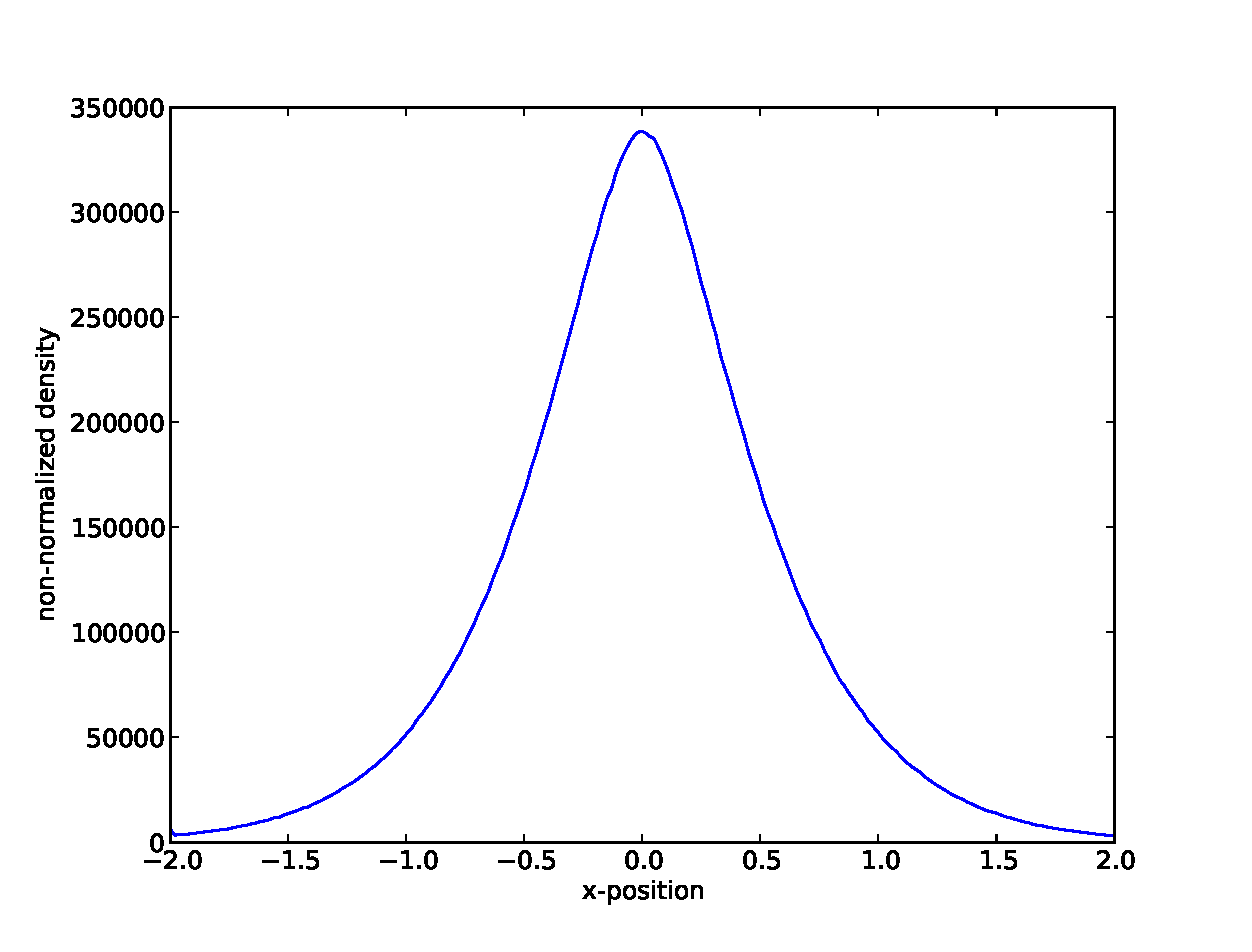
\includegraphics[width=6cm]{figures/densities/Hex.eps}
	\label{fig:subfig62}
}
\subfigure[projection on the xy-plane]{
	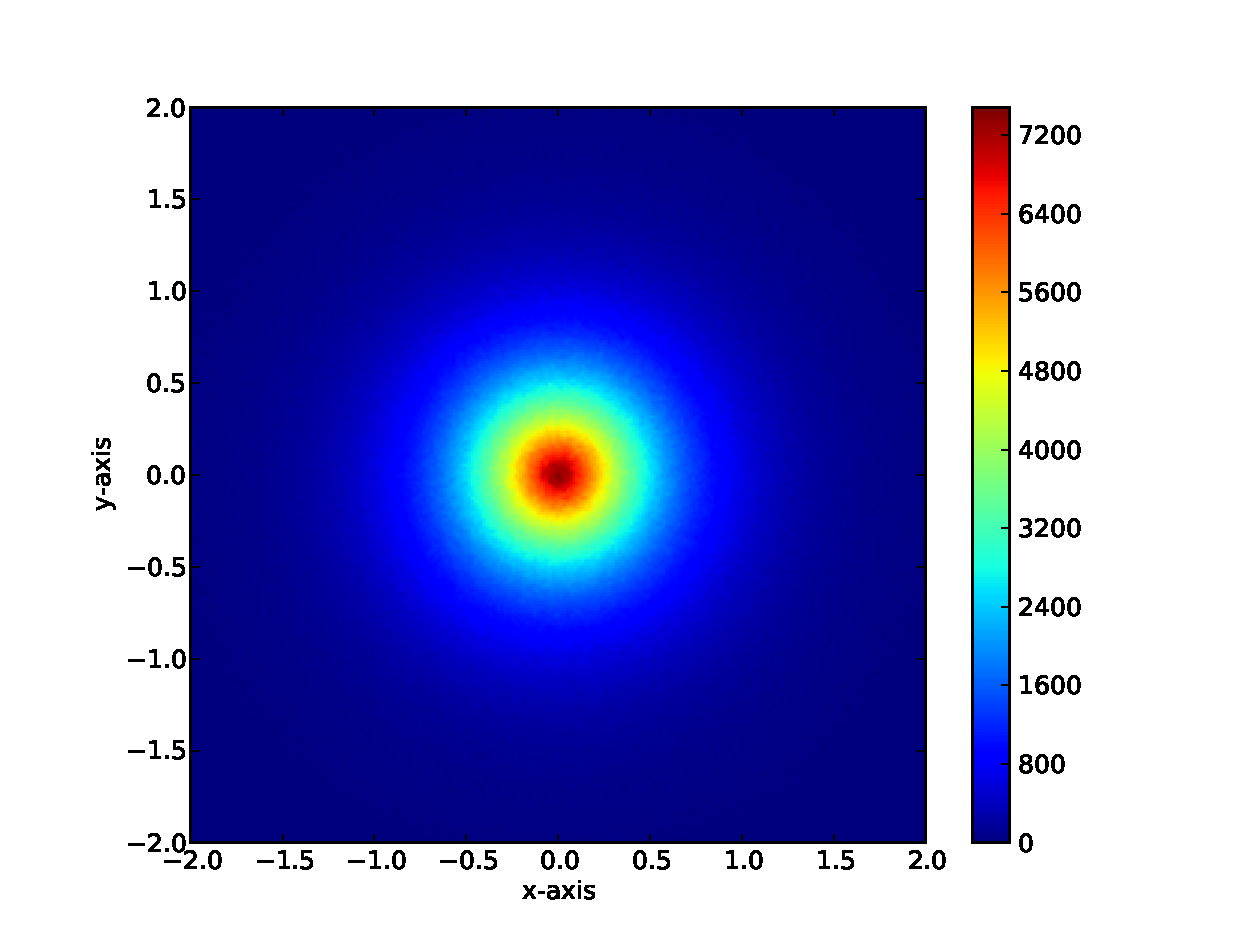
\includegraphics[width=7cm]{figures/densities/Hexy.eps}
	\label{fig:subfig63}
}
\subfigure[3d distribution]{
	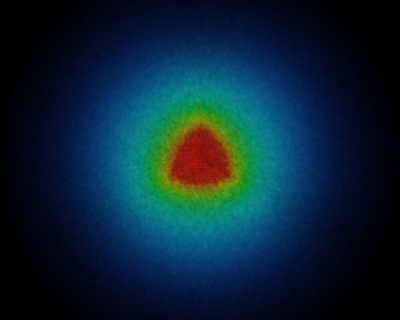
\includegraphics[width=6cm]{figures/densities/Hexyz.png}
	\label{fig:subfig64}
}
\caption[Optional caption for list of figures]{The figures show various projections of the non-normalized one-body density of He. The radial distribution shows pure hydrogenic orbitals, optimization over $\alpha$ only, optimization over $\beta$ only, and complete optimization. The rest show only the complete optimization.}
\label{fig:6}
\end{figure}

\begin{figure}[ht]
\subfigure[radial distribution]{
	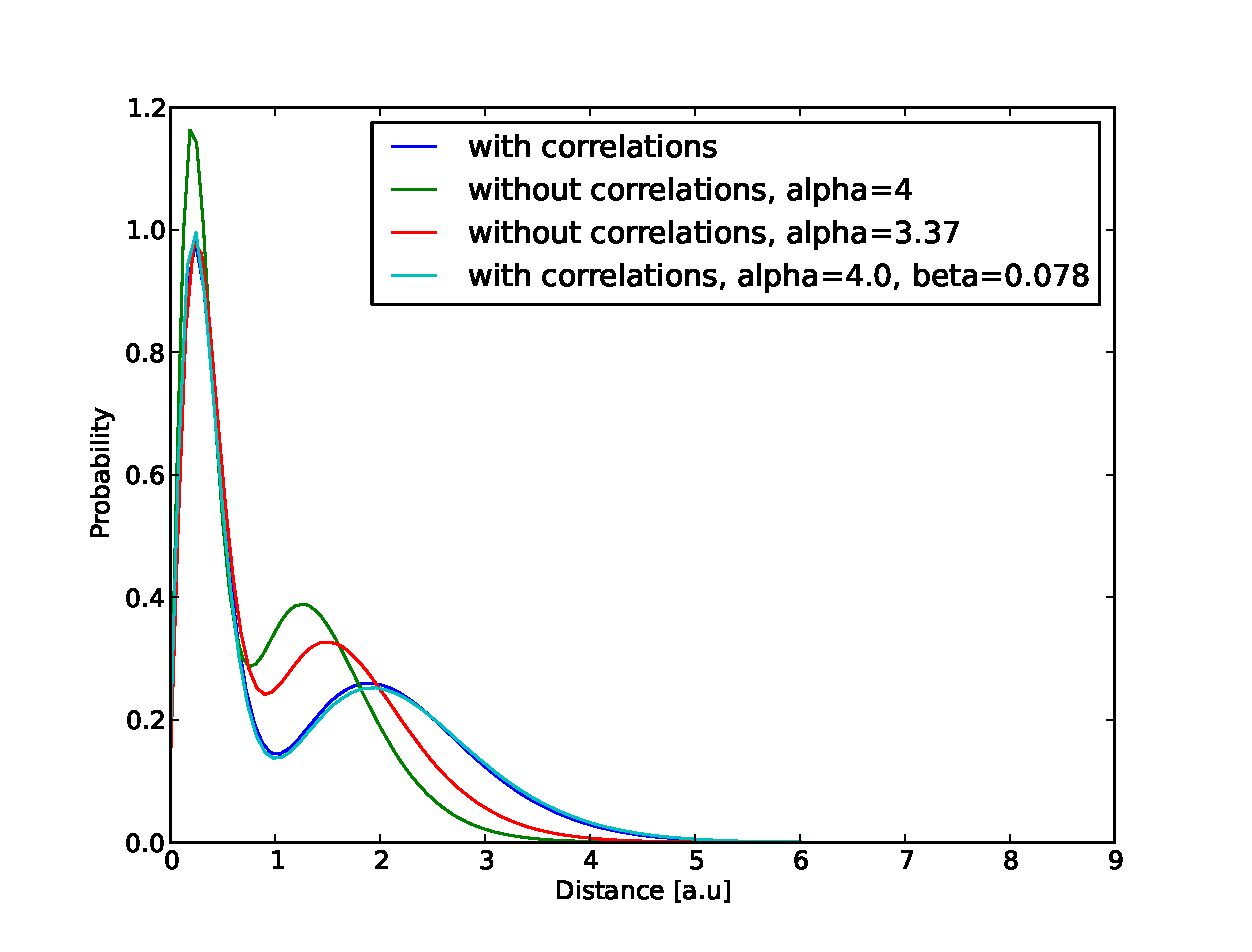
\includegraphics[width=6cm]{figures/densities/Berad.eps}
	\label{fig:subfig71}
}
\subfigure[projection on the x-axis]{
	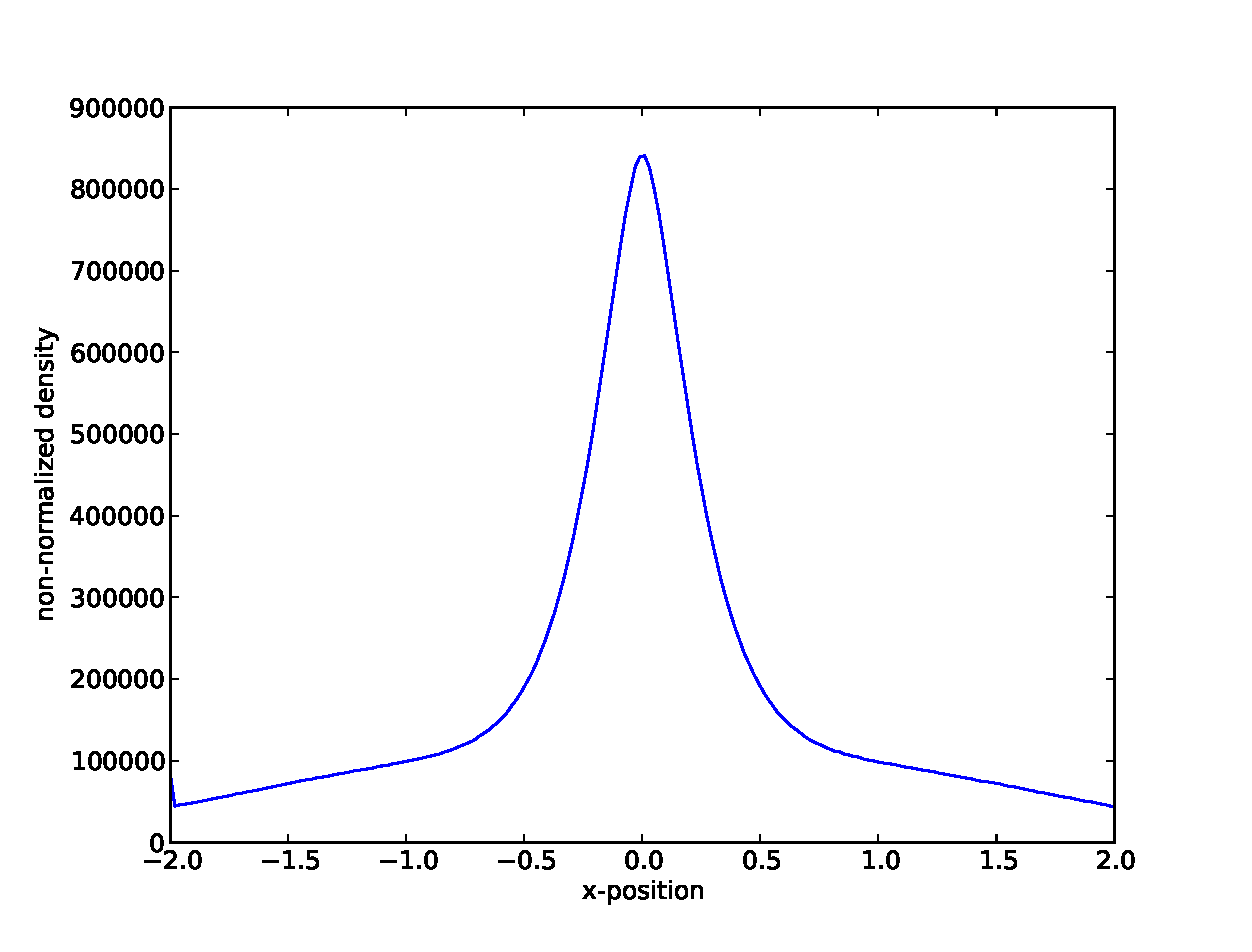
\includegraphics[width=6cm]{figures/densities/Bex.eps}
	\label{fig:subfig72}
}
\subfigure[projection on the xy-plane]{
	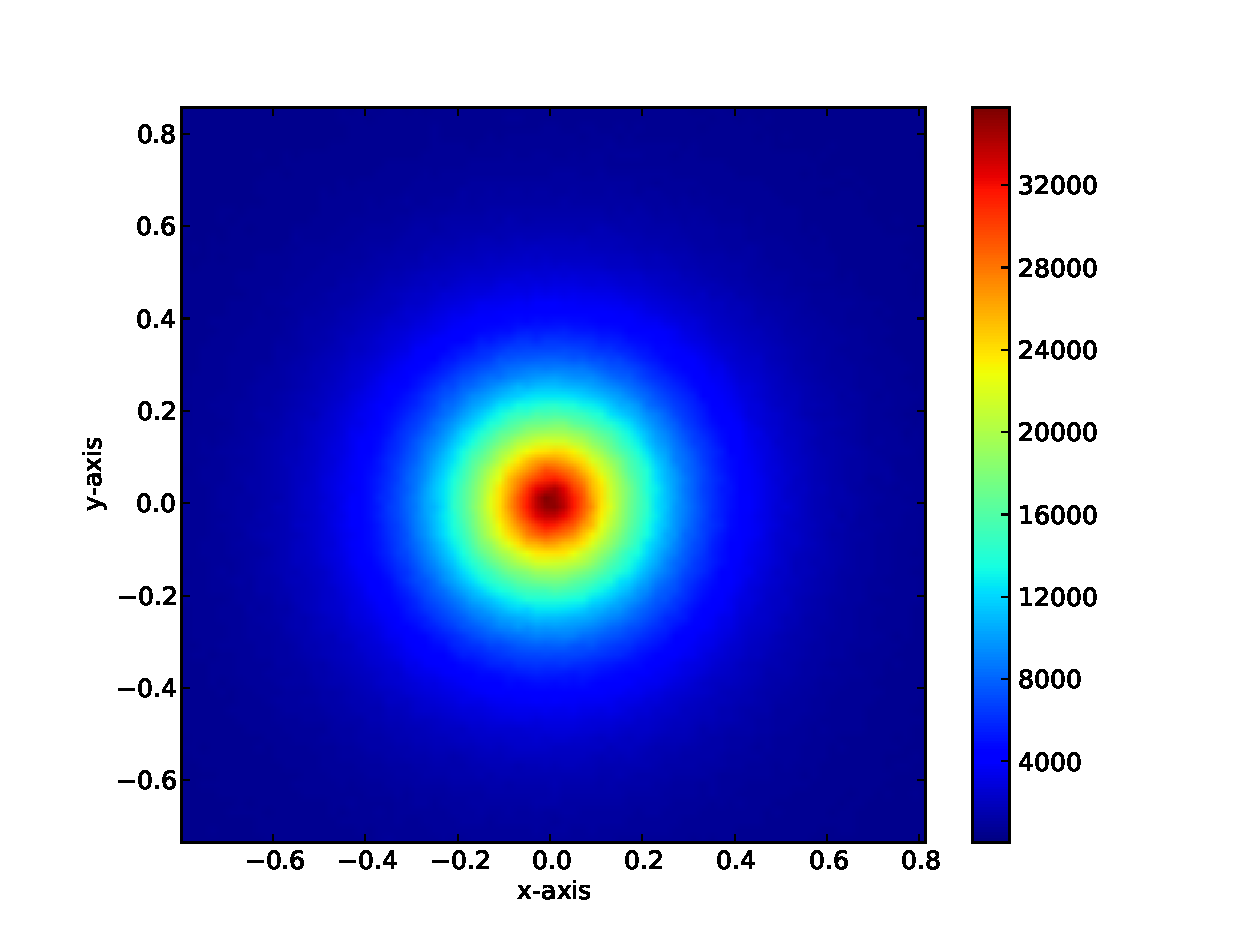
\includegraphics[width=7cm]{figures/densities/Bexy.eps}
	\label{fig:subfig73}
}
\subfigure[3d distribution]{
	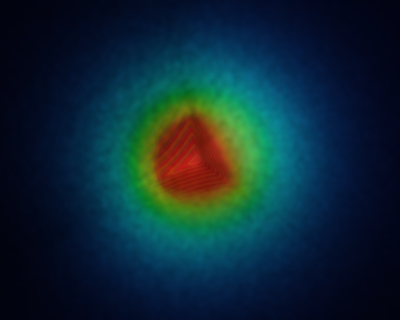
\includegraphics[width=6cm]{figures/densities/Bexyz.png}
	\label{fig:subfig74}
}
\caption[Optional caption for list of figures]{The figures show various projections of the non-normalized one-body density of Be. The radial distribution shows pure hydrogenic orbitals, optimization over $\alpha$ only, optimization over $\beta$ only, and complete optimization. The rest show only the complete optimization.}
\label{fig:7}
\end{figure}

\begin{figure}[ht]
\subfigure[radial distribution]{
	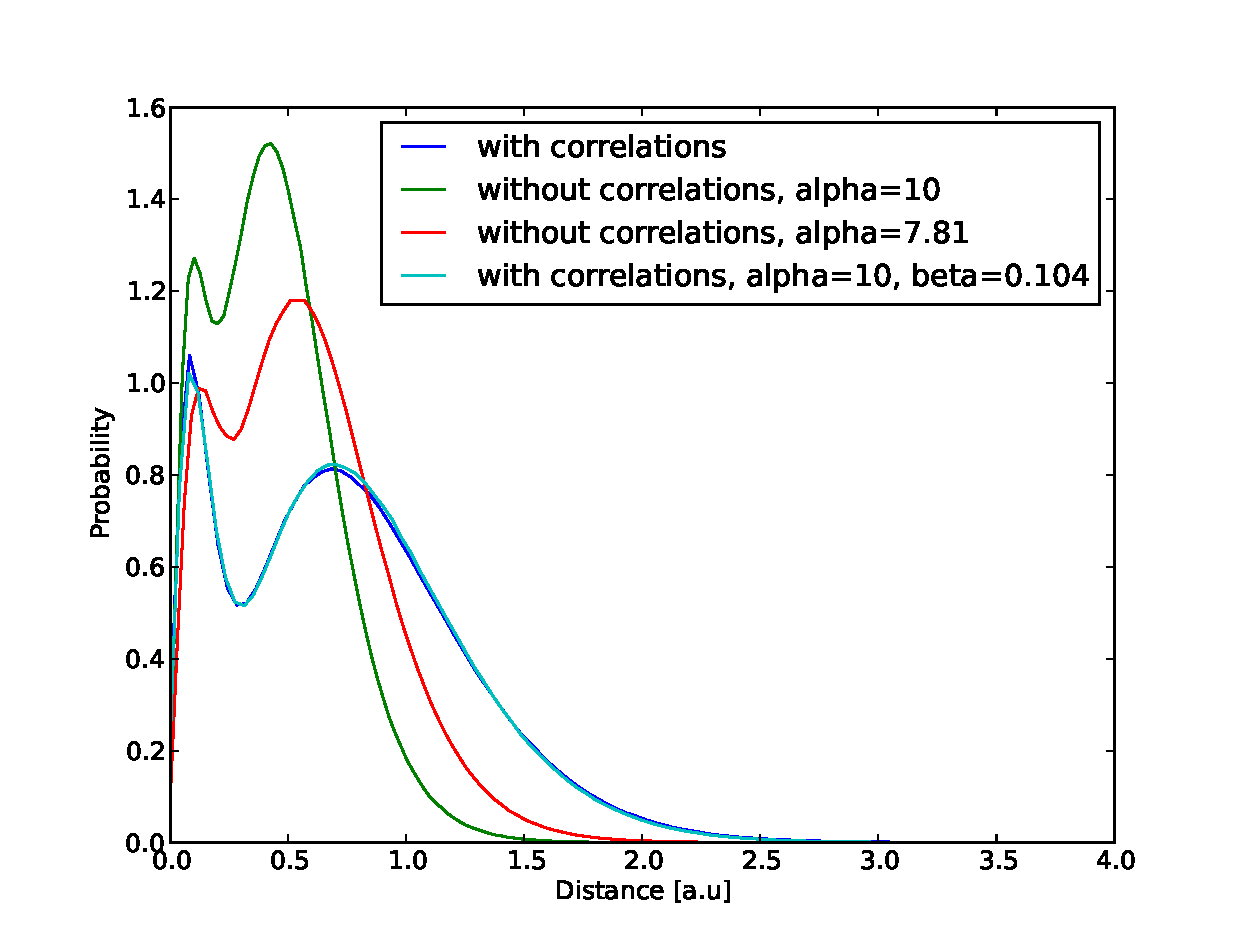
\includegraphics[width=6cm]{figures/densities/Nerad.eps}
	\label{fig:subfig81}
}
\subfigure[projection on the x-axis]{
	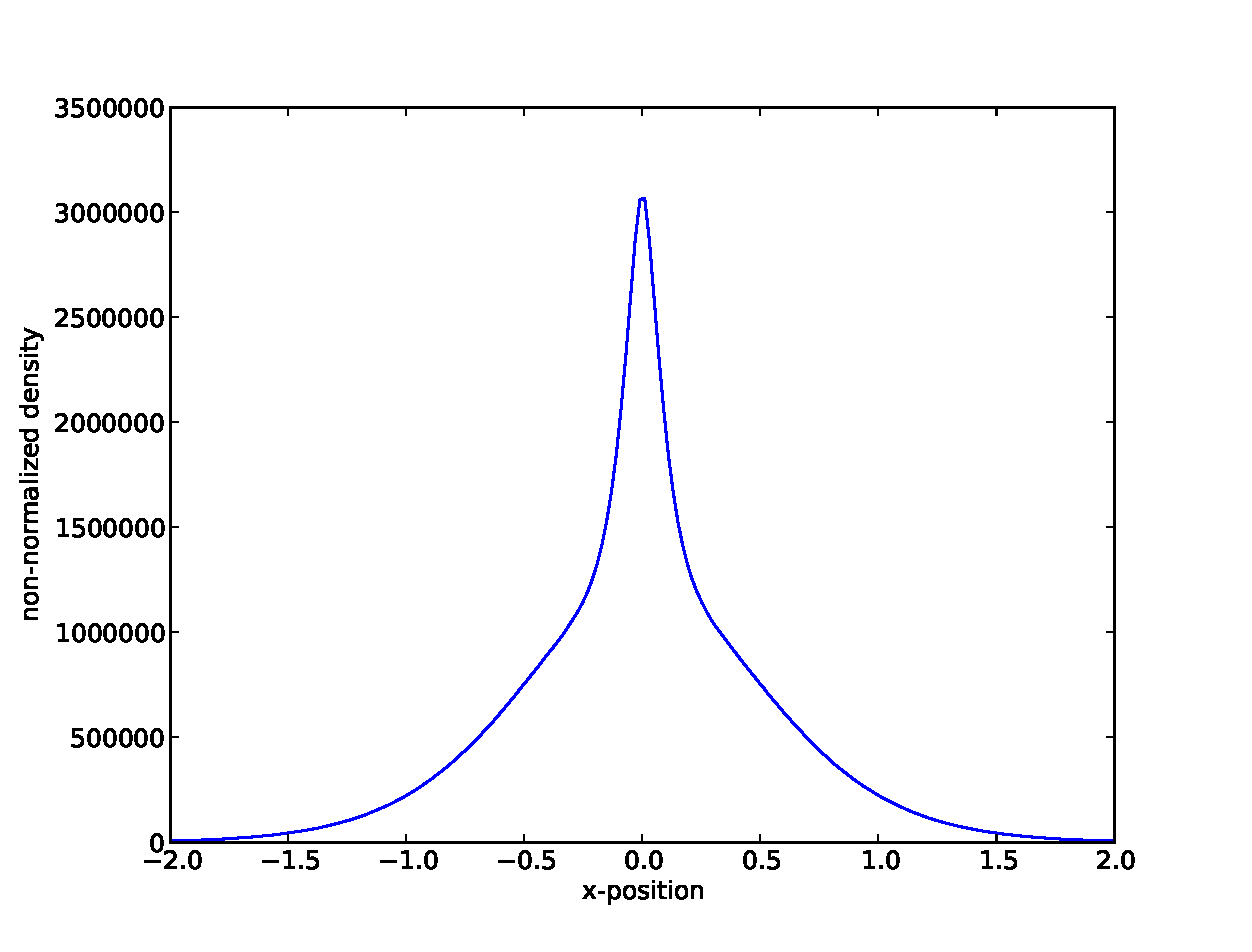
\includegraphics[width=6cm]{figures/densities/Nex.eps}
	\label{fig:subfig82}
}
\subfigure[projection on the xy-plane]{
	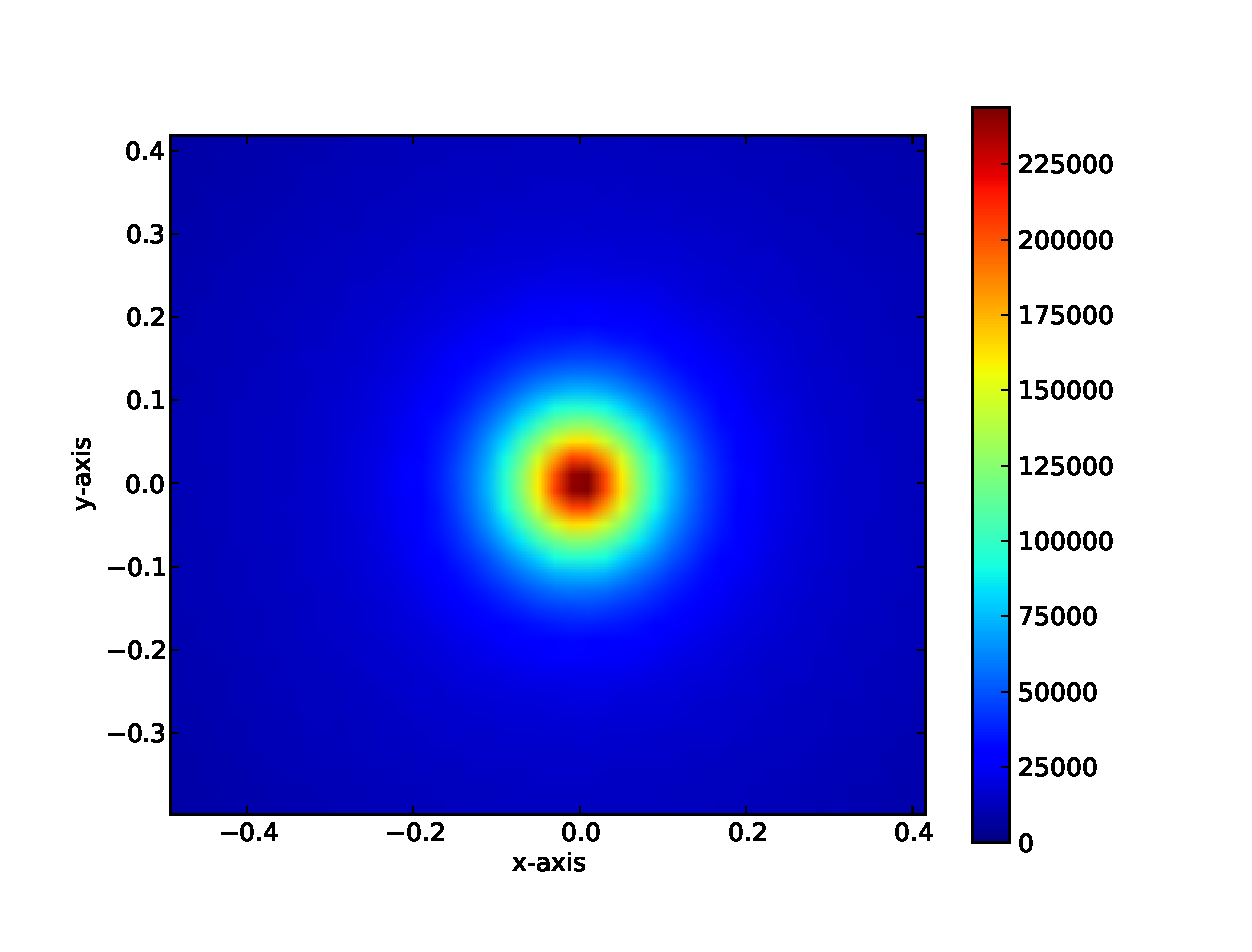
\includegraphics[width=7cm]{figures/densities/Nexy.eps}
	\label{fig:subfig83}
}
\subfigure[3d distribution]{
	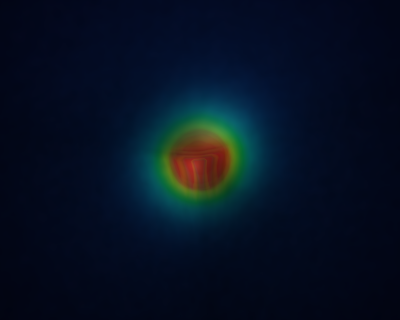
\includegraphics[width=6cm]{figures/densities/Nexyz.png}
	\label{fig:subfig84}
}
\caption[Optional caption for list of figures]{The figures show various projections of the non-normalized one-body density of Ne. The radial distribution shows pure hydrogenic orbitals, optimization over $\alpha$ only, optimization over $\beta$ only, and complete optimization. The rest show only the complete optimization.}
\label{fig:8}
\end{figure}

\label{sec:densities}
\begin{figure}[ht]
\subfigure[radial distribution]{
	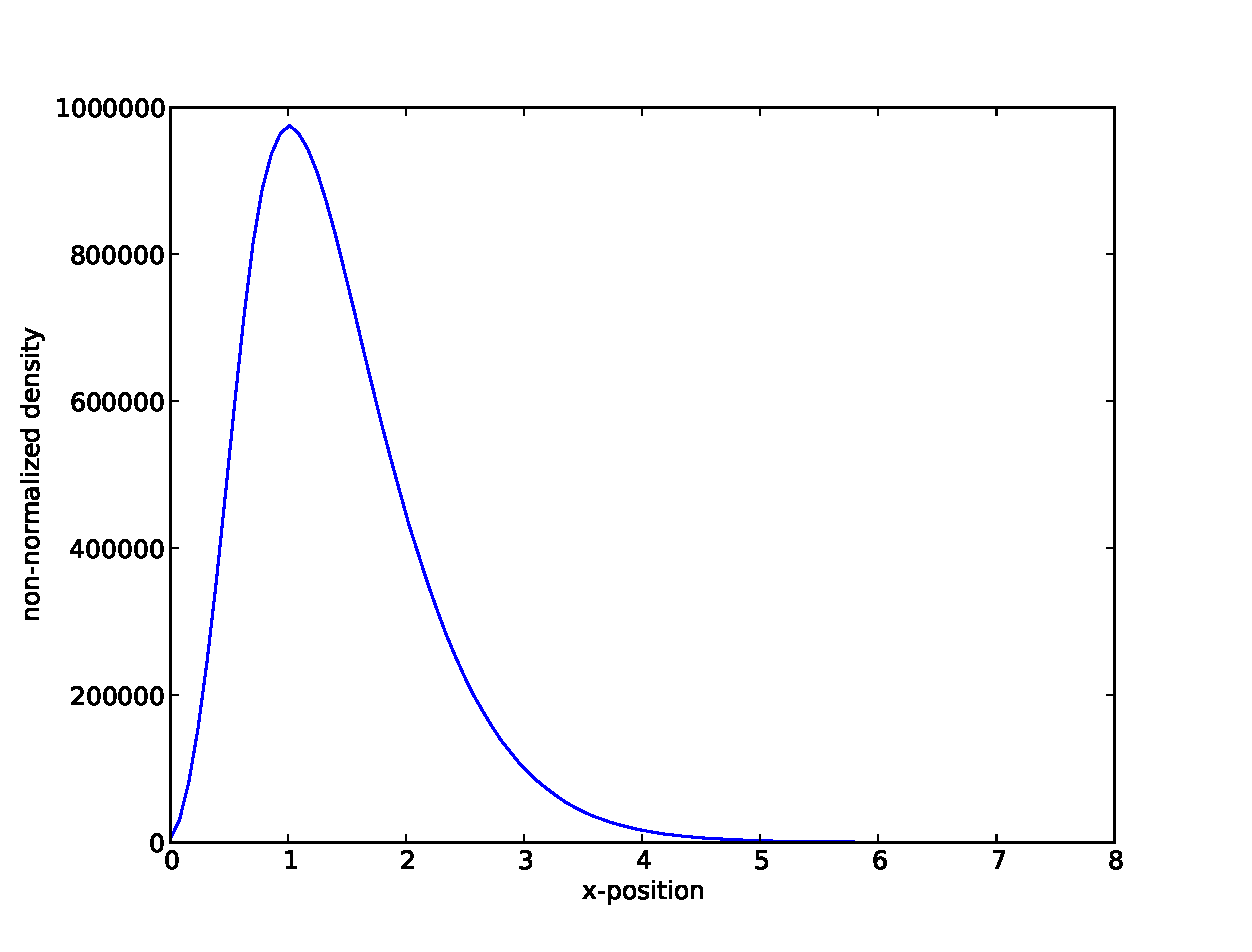
\includegraphics[width=6cm]{figures/densities/H2rad.eps}
	\label{fig:subfig91}
}
\subfigure[projection on the x-axis]{
	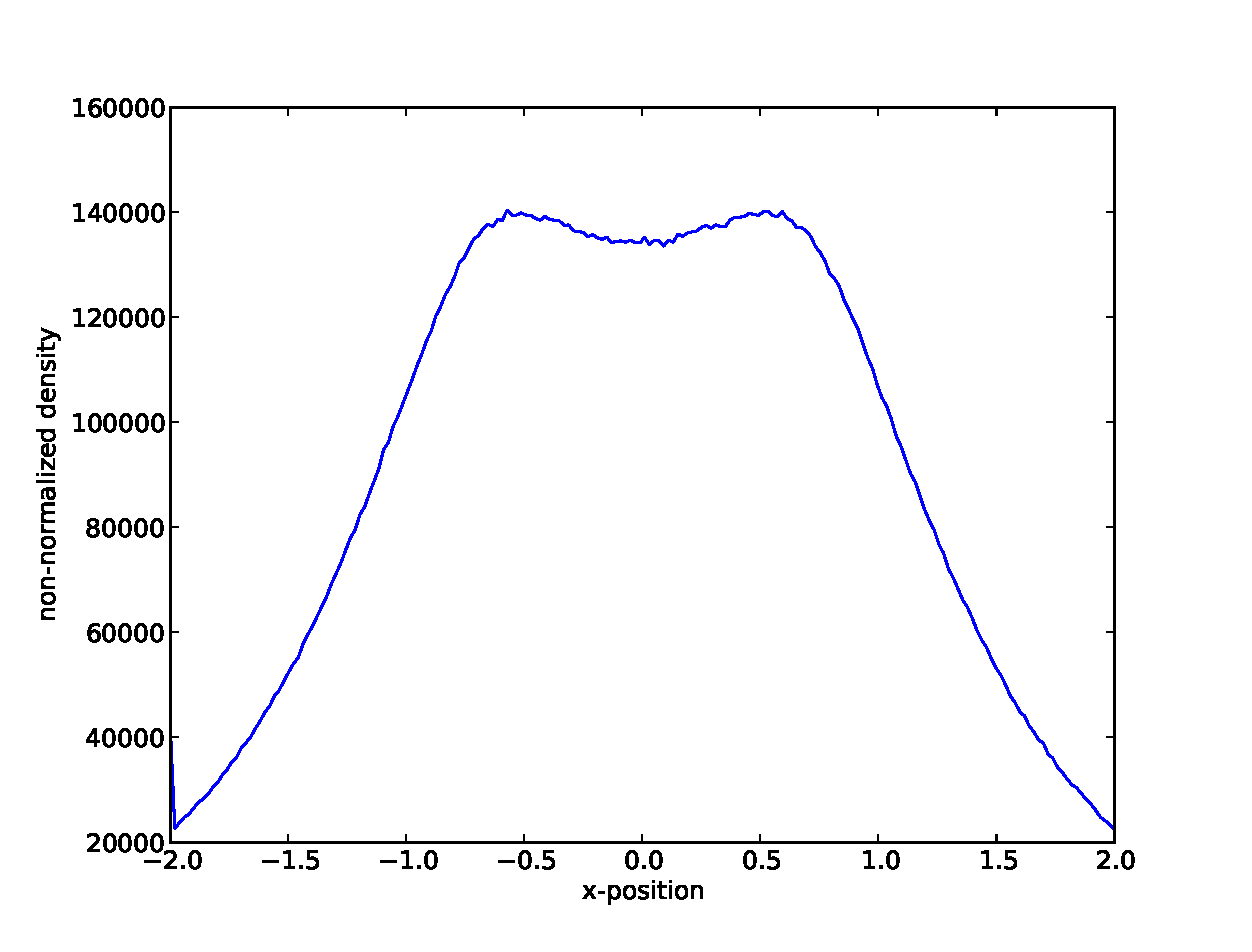
\includegraphics[width=6cm]{figures/densities/H2x.eps}
	\label{fig:subfig92}
}
\subfigure[projection on the xy-plane]{
	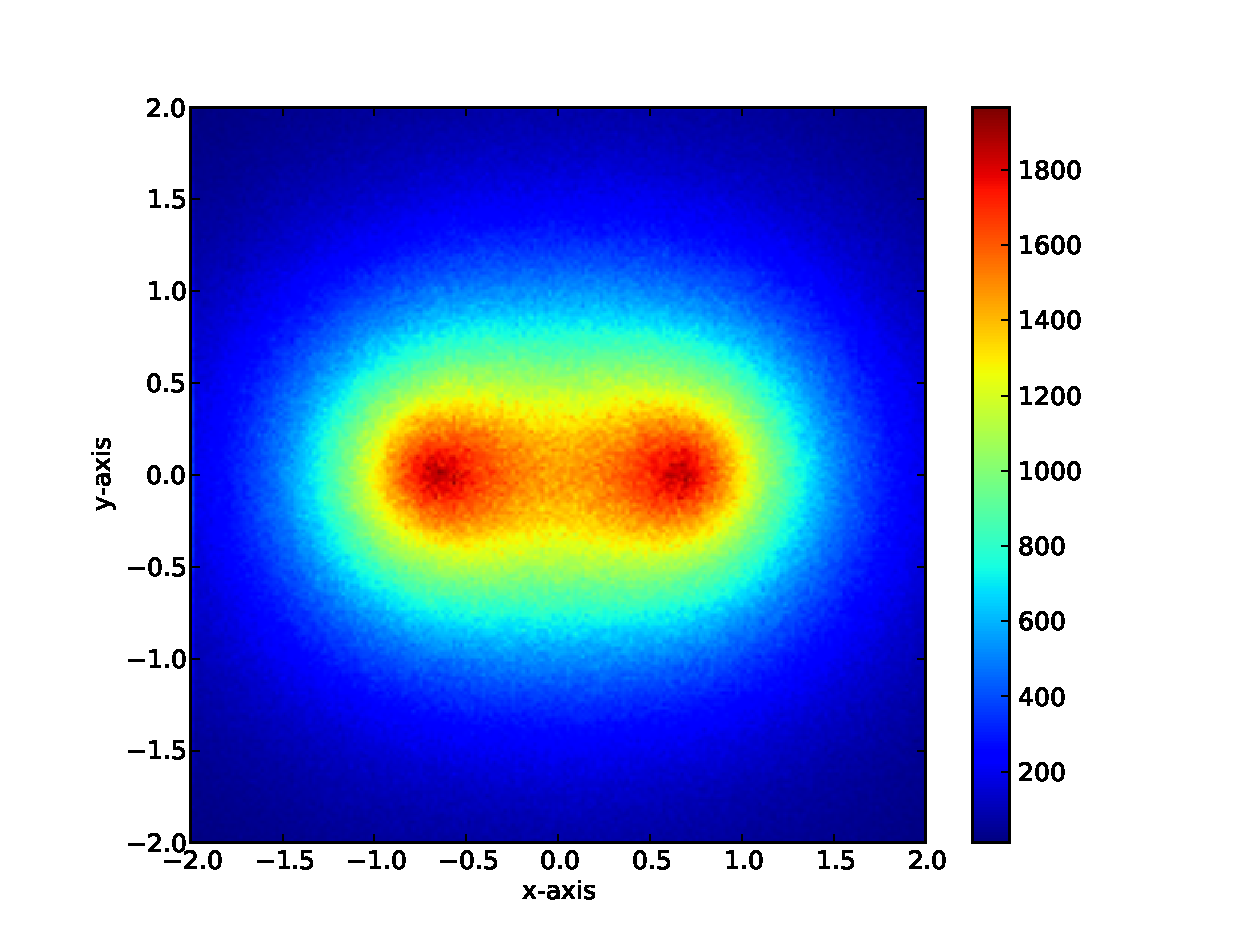
\includegraphics[width=7cm]{figures/densities/H2xy.eps}
	\label{fig:subfig93}
}
\subfigure[3d distribution]{
	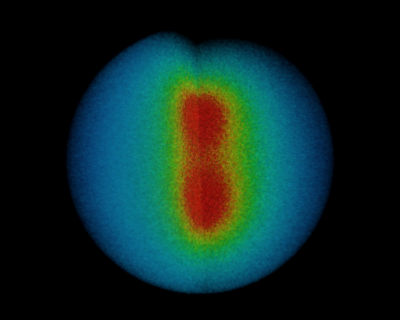
\includegraphics[width=6cm]{figures/densities/H2xyz.png}
	\label{fig:subfig94}
}
\caption[Optional caption for list of figures]{The figures show various projections of the non-normalized one-body density of $\text{H}_2$.}
\label{fig:9}
\end{figure}

\begin{figure}[ht]
\subfigure[radial distribution]{
	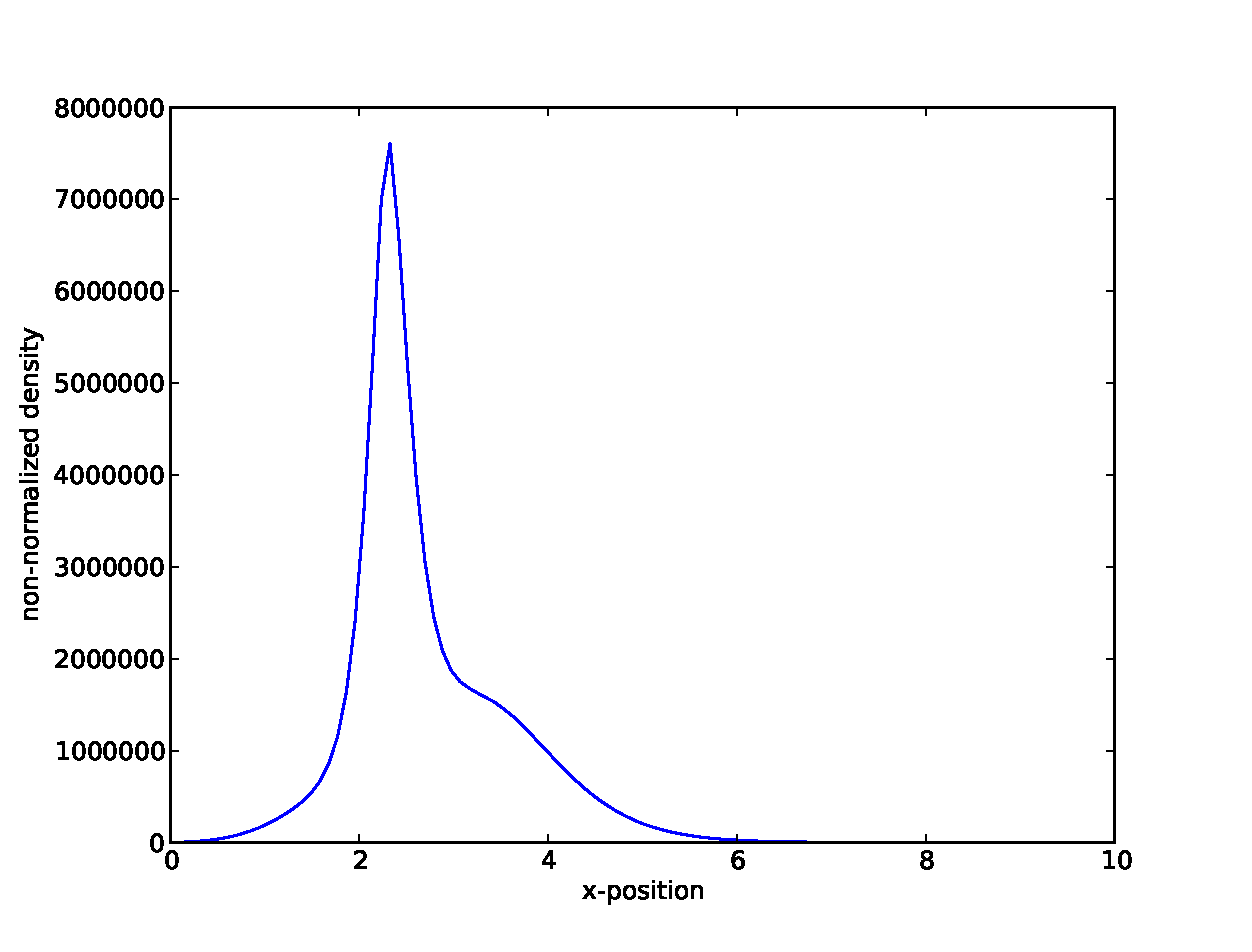
\includegraphics[width=6cm]{figures/densities/Be2rad.eps}
	\label{fig:subfig101}
}
\subfigure[projection on the x-axis]{
	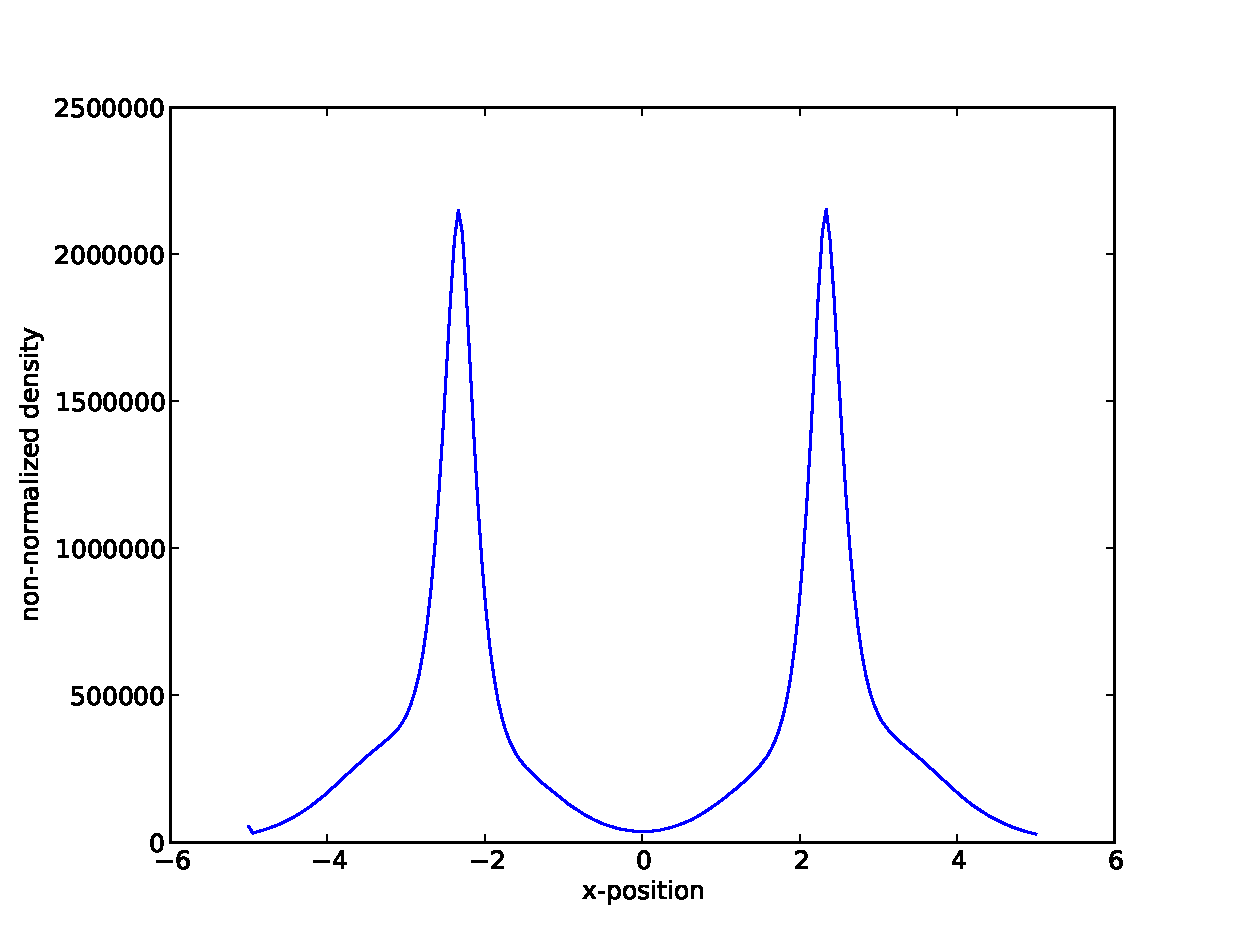
\includegraphics[width=6cm]{figures/densities/Be2x.eps}
	\label{fig:subfig102}
}
\subfigure[projection on the xy-plane]{
	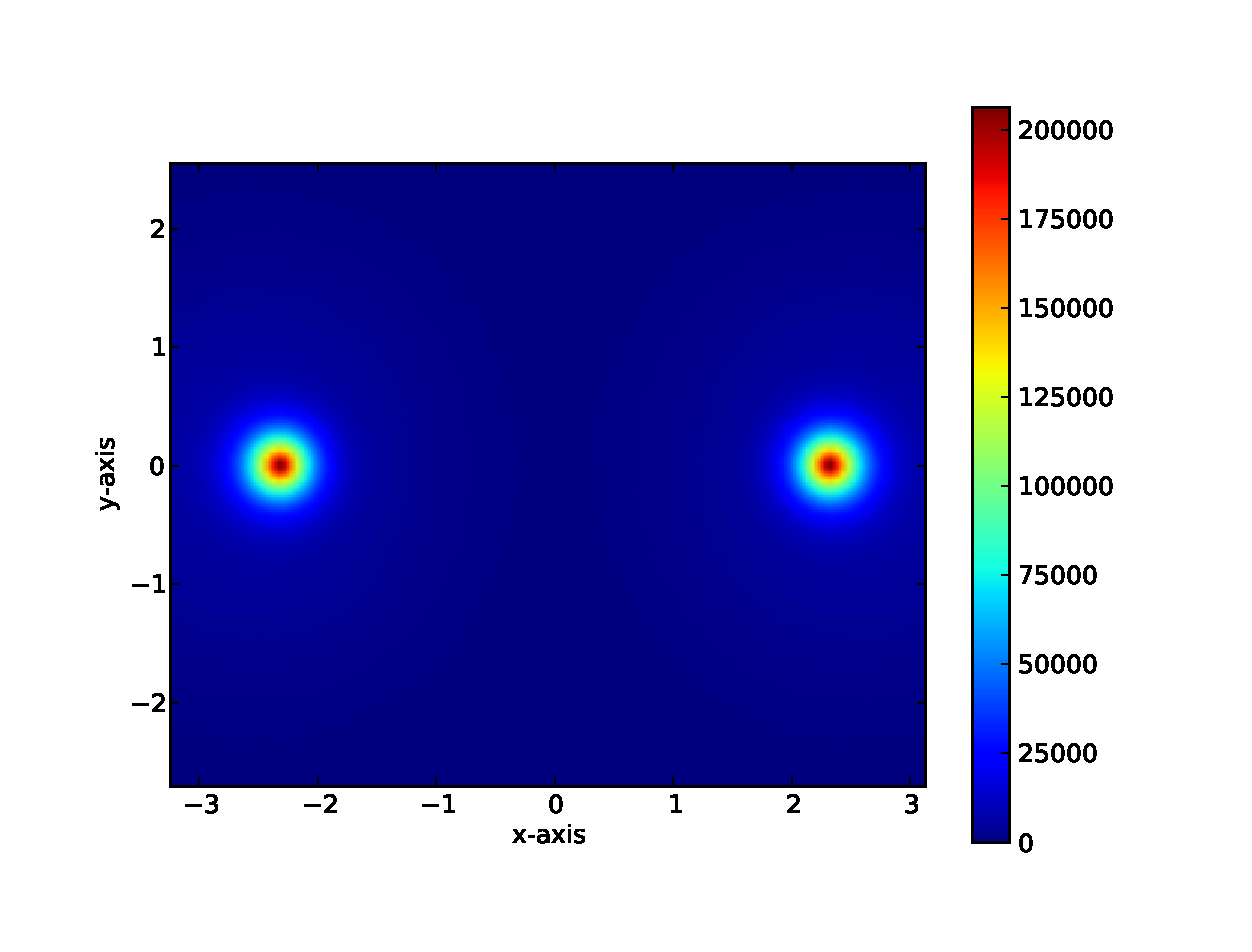
\includegraphics[width=7cm]{figures/densities/Be2xy.eps}
	\label{fig:subfig103}
}
\subfigure[3d distribution]{
	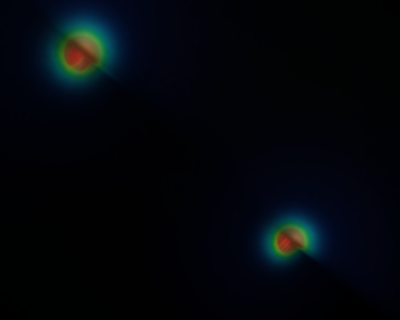
\includegraphics[width=6cm]{figures/densities/Be2xyz.png}
	\label{fig:subfig104}
}
\caption[Optional caption for list of figures]{The figures show various projections of the non-normalized one-body density of $\text{Be}_2$.}
\label{fig:10}
\end{figure}
\clearpage



\section{Conclutions and perspectives}
I have developed an object oriented code for doing VMC calculations of quantum systems. This includes parameter optimization search and statistical analysis, as well as the Metropolis algorithm with importance sampling for doing the main VMC calculations. The code runs the single Monte Carlo calculations in parallel using MPI, and the broad spectre brute force optimization using OpenMP.  

Future work would involve generalizing the code further (see Appendix \ref{sec:code} for  details on the current structure of the code). This would invole making a Hamiltonian class to allow for arbitrary potentials, as well as making the program easier to use (perhaps by including a wrapper in python or using some GUI). It would also by within reason to give the code a complete makeover, to ensure the different modules communicate better.

\section*{Acknowledgments}

I would like to thank the instructors at the group for Computational Physics and the University of Oslo for many illuminating discussions, and in particular Jørgen Høgberget for providing useful results from VMC and DMC for benchmarking. 

\begin{appendices}
 \section{Program code}
 \label{sec:code}
 For the project I made an object oriented code, the program consists of the following classes: 
\begin{itemize}
 \item \verb Atom . This essentially contains physical info such as the number of particles, the charge, whether the particle is an atom or a molecule etc.

 \item \verb VMCSetup . The purpose of this function is to set up the different kinds of program runs, such as parameter optimization, production runs, etc. 
 
 \item \verb VMCSolver . This is created by \verb VMCSetup , and does the actual Monte Carlo integration, using the Metropolis algorithm (with or without importance sampling)
 
 \item \verb WaveFunction . This class creates the slater determinant and the jastrow (optional), and collects the values of wavefunctions, gradients and laplacians from these. 
 
 \item \verb SlaterDeterminant . Creates a vector of \verb Orbital  objects, and is used to calculate the value of the slater determinant, and its gradients and laplacians. 
 
 \item \verb Jastrow . Calculates the value, gradients and laplacians of the correlation part of the wave function.
 
 \item \verb Orbital . This is called by \verb SlaterDeterminant , and creates the single particles wave functions which makes up the determinant as well as the single particle gradients and laplacians used by functions in the SlaterDeterminant class. 
 
 \item \verb MoleculeOrbital  \verb inherits  \verb Orbital , the molecule version of \verb Orbital .
 
 \item \verb Blocking . Not a part of the rest of the program. Uses data collected from runs to calculate the standard error using the blocking method. 
\end{itemize}
And overview of program calls is shown in figure \ref{fig:11}. The code is available at https://github.com/andreavs/fys4411/tree/master/VMC.

\begin{widetext}
\begin{figure}
\centering
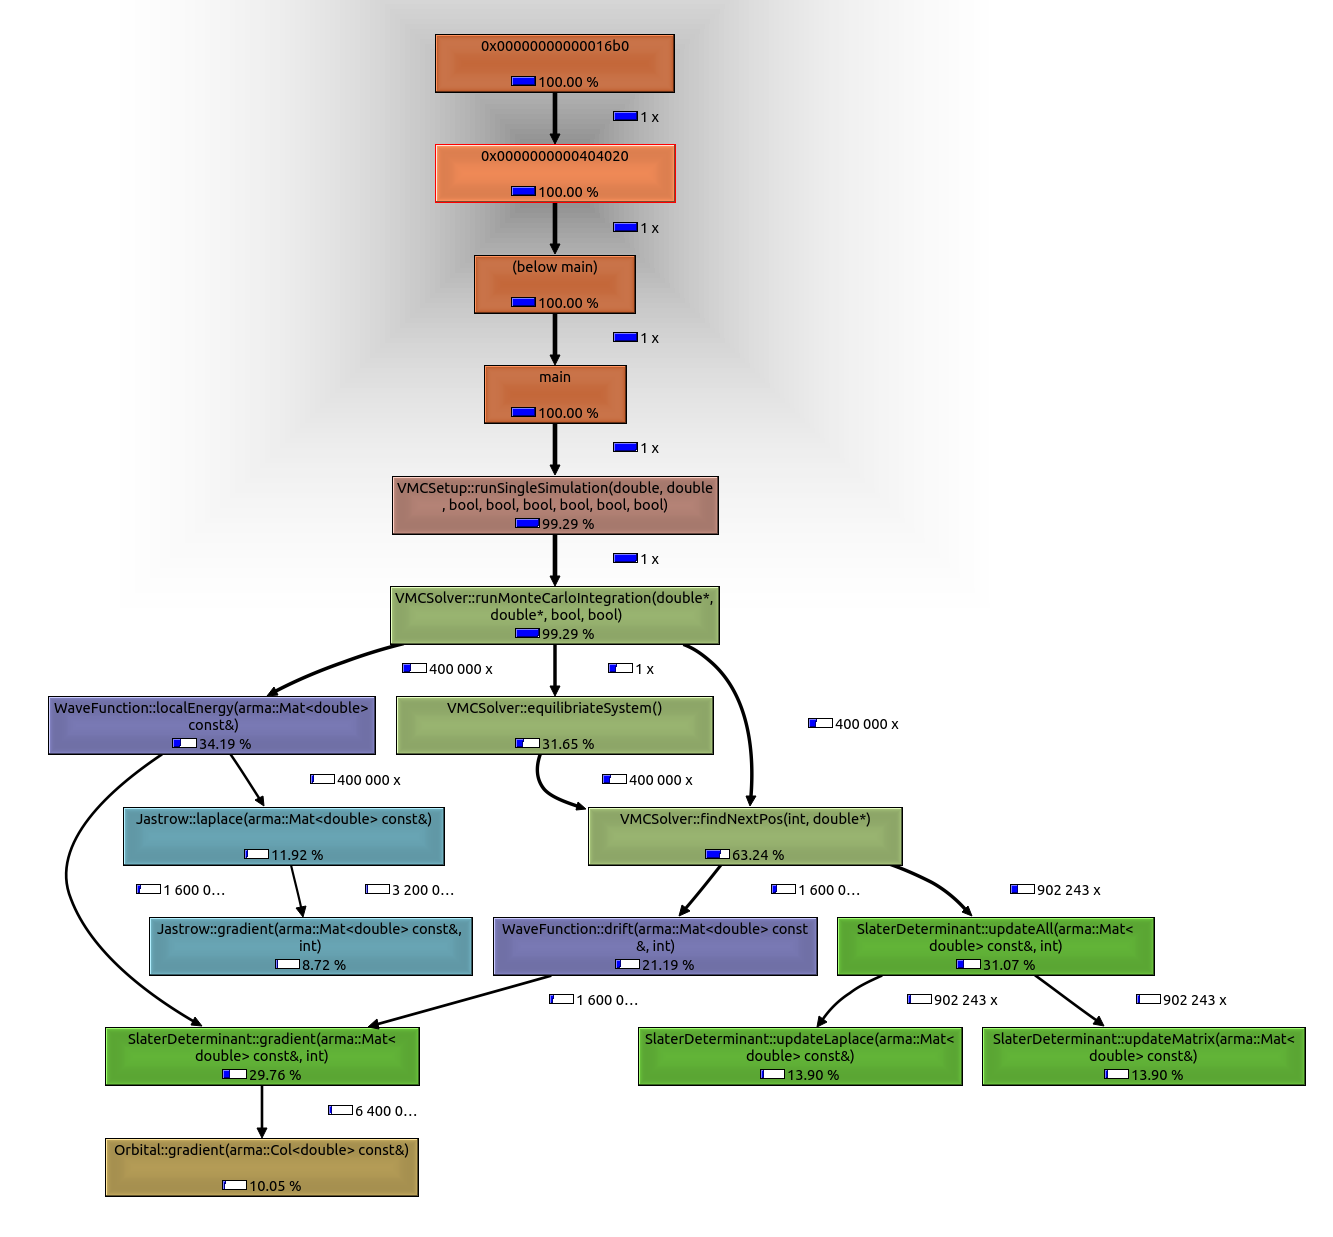
\includegraphics[width=17cm]{figures/programview.png}
\caption{\label{fig:11} The figure shows the overview of the a typical program run}
\end{figure}
\end{widetext}
 
 
 \section{Expressions for gradients and laplacians}
 \label{sec:gradlap}
 When implementing the closed form expression for the energy earlier, we calculated 
\begin{equation}
 {1 \over \psi_T} \hat{H} \psi_T
\end{equation}
where the tricky part was calculating the $\nabla^2_1\psi$ term. Let us see if we are able to calculate this term in our more general case. Our wavefunction can be factorized as 
\begin{equation}
 \psi_T(\{ \rvec_i \}) = \psi_S(\{ \rvec_i \})\psi_C(\{\rvec_i \})
\end{equation}
where $\psi_S$ is the Slater Determinant, and $\psi_C$ contains the jastrow factor. In this way, we can write the laplacian as 
\begin{equation}
 \nabla_i^2 \psi_S \psi_T = \psi_C \nabla_i^2 \psi_S + 2 \nabla_i \psi_S \cdot \nabla_i \psi_S + \psi_S \nabla_i^2 \psi_C^2
\end{equation}
This as the combined advantage of being close to how we would want to implement the closed form expressions, and making the derivations to come more digestable. Lets get to work. We'll start with the jastrow factor, and the results will be summarized in table \ref{tab:2}. We begin by noting that
\begin{widetext}
\begin{align}
 {\partial \over \partial x_i} \psi_C & =  {\partial \over \partial x_i}\prod_{j<k}^n \exp\left( { a_{jk} r_{jk} \over 1 + \beta r_{jk}} \right) \\
 & =  {\partial \over \partial x_i} \exp \left( \sum_{j<k}^n { a_{jk} r_{jk} \over 1 + \beta r_{jk}}\right) \\
 & = \left( \sum_{j \ne i} { a_{ij}(x_i - x_j) \over r_{ij}(\beta r_{ij} + 1)^2} \right) \psi_C
\end{align}
which can be generalized as 
\begin{equation}
 \nabla_i \psi_C = \left( \sum_{j \ne i} { a_{ij}(\rvec_i - \rvec_j) \over r_{ij}(\beta r_{ij} + 1)^2} \right) \psi_C
\end{equation}
Going further, using the product rule, we have that 
\begin{align}
 {\partial^2 \over \partial x_i^2} \psi_C & = \left[ \left( \sum_{j \ne i} { a_{ij}(x_i - x_j) \over r_{ij}(\beta r_{ij} + 1)^2} \right)^2  + {\partial \over \partial x_i} \left( \sum_{j \ne i} { a_{ij}(x_i - x_j) \over r_{ij}(\beta r_{ij} + 1)^2} \right)   \right] \psi_C \\
 & = \left[ \left( \sum_{j \ne i} { a_{ij}(x_i - x_j) \over r_{ij}(\beta r_{ij} + 1)^2} \right)^2  + \sum_{j \ne i}\left(  { a_{ij} \over r_{ij}(\beta r_{ij} + 1)^2} - {a_{ij}(x_i-x_j)^2(3\beta r_{ij} + 1) \over r_{ij}^3(\beta r_{ij} + 1)^3 } \right)  \right] \psi_C \\
 & = \sum_{j\ne i}\left[  { a_{ij}^2(x_i - x_j)^2 \over r_{ij}^2(\beta r_{ij} + 1)^4} + { a_{ij} \over r_{ij}(\beta r_{ij} + 1)^2} - {a_{ij}(x_i-x_j)^2(3\beta r_{ij} + 1) \over r_{ij}^3(\beta r_{ij} + 1)^3}\right.\\
 & + \left.2\sum_{k \ne j} {a_{ij}a_{ik} (x_i-x_j)(x_i - x_k) \over r_{ij}r_{ik}(\beta r_{ij} + 1)^2(\beta r_{jk} + 1)^2  } \right]\psi_C
\end{align}
and we can generalize this to 
\begin{align}
 \nabla_i^2 \psi_C &= \sum_{j\ne i}\left[  { a_{ij}^2 \over (\beta r_{ij} + 1)^4} + { 3a_{ij} \over r_{ij}(\beta r_{ij} + 1)^2} - {a_{ij}(3\beta r_{ij} + 1) \over r_{ij}(\beta r_{ij} + 1)^3}\right.\\
 & + \left.2\sum_{k \ne j} {a_{ij}a_{ik} (\rvec_i-\rvec_j)\cdot(\rvec_i - \rvec_k) \over r_{ij}r_{ik}(\beta r_{ij} + 1)^2(\beta r_{jk} + 1)^2  } \right]\psi_C \\
 &= \sum_{j\ne i}\left[  { a_{ij}^2 \over (\beta r_{ij} + 1)^4} +  {2a_{ij} \over r_{ij}(\beta r_{ij} + 1)^3} + 2\sum_{k \ne j} {a_{ij}a_{ik} (\rvec_i-\rvec_j)\cdot(\rvec_i - \rvec_k) \over r_{ij}r_{ik}(\beta r_{ij} + 1)^2(\beta r_{jk} + 1)^2  } \right]\psi_C
\end{align}
And so, to avoid redundant calculations, we can write the sum of the laplacians as
\begin{equation}
 \sum_{i} \nabla_i^2 \psi_C = 2 \sum_i \sum_{j>i}  {a_{ij}\over (\beta r_{ij} + 1)^2}\left[  { a_{ij} \over (\beta r_{ij} + 1)^2} +  {2 \over r_{ij}(\beta r_{ij} + 1)} + 4\sum_{k > j} {a_{ik} (\rvec_i-\rvec_j)\cdot(\rvec_i - \rvec_k) \over r_{ij}r_{ik}(\beta r_{jk} + 1)^2  } \right]\psi_C
\end{equation}
 \end{widetext}
For the slater determinant, if we denote the matrix by $\mathcal{D}$, then its gradient is given by Jacobi's formula as
\begin{equation}
 \nabla_i |\mathcal{D}(\rvec)| = |\mathcal{D}(\rvec)| \sum_{j=0}^n \nabla_i d_{ij}(\rvec) d_{ij}^{-1}(\rvec)
\end{equation}
where $d_{ij}$ is the $ij$-element of $\mathcal{D}$ and $d_{ij}^{-1}$ is the $ij$-element of $\mathcal{D}^{-1}$. The laplacian is
\begin{equation}
 \nabla_i^2 |\mathcal{D}(\rvec)| = |\mathcal{D}(\rvec)| \sum_{j=0}^n \nabla_i^2 d_{ij}(\rvec) d_{ij}^{-1}(\rvec)
\end{equation}



We should calculate the gradients and laplacians of the relevant wave functions as well, we'll start with the 1s state, $\phi_{1s}(\rvec) = \exp(-\alpha r)$. 
\begin{equation}
 \nabla \phi_{1s}(\rvec) = {- \alpha \rvec  \exp(-\alpha r) \over r}
\end{equation}
and 
\begin{equation}
 \nabla^2 \phi_{1s}(\rvec) = \alpha (\alpha r - 2)\exp(-\alpha r)/r,
\end{equation}
These computations get tedious, and we should utilize some symbolic software such as sumpy to avoid human errors. The rest of the wave function results are summarized in table \ref{tab:2}.


\begin{widetext}
\begin{table}[!ht]
\centering

\begin{tabular}{|c|c|c|}
 \hline
 function & gradient & laplacian \\
 \hline
 $\phi_{1s}(\rvec)$ & $\alpha \rvec \phi_{1s}/ r $ & $\alpha (\alpha r - 2)\phi_{1s}/r$ \\
 $\phi_{2s}(\rvec)$ & $\alpha \rvec (\alpha r - 4) \exp(-\alpha r/2)/4r$ & $-\alpha(\alpha^2r^2 - 10r\alpha + 16)\exp(-\alpha r/2)/8r$ \\
 & & \\
 $\phi_{2px}(\rvec)$ & $-\alpha(\alpha x^2 - 2r,\alpha x y ,\alpha xz )\exp(-\alpha r/2)/(2r)$ & $\alpha^2x (\alpha r - 8) \exp(-\alpha r/2)/4r$  \\
  $\phi_{2py}(\rvec)$ & $-\alpha(\alpha x y, \alpha y^2 - 2r,\alpha yz )\exp(-\alpha r/2)/(2r)$ & $\alpha^2y (\alpha r - 8) \exp(-\alpha r/2)/4r$  \\
   $\phi_{2pz}(\rvec)$ & $-\alpha(\alpha xz, \alpha yz, \alpha z^2 - 2r )\exp(-\alpha r/2)/(2r)$ & $\alpha^2z (\alpha r - 8) \exp(-\alpha r/2)/4r$  \\
   & & \\ 
   $\psi_C$ & $\nabla_i \psi_C = \left( \sum_{j \ne i} { a_{ij}(\rvec_i - \rvec_j) \over r_{ij}(\beta r_{ij} + 1)^2} \right) \psi_C$ &  $2  \sum_{j>i}  {a_{ij}\over (\beta r_{ij} + 1)^2}\left[  { a_{ij} \over (\beta r_{ij} + 1)^2} +  {2 \over r_{ij}(\beta r_{ij} + 1)}\right.$ \\
   & & $+ \left. 4\sum_{k > j} {a_{ik} (\rvec_i-\rvec_j)\cdot(\rvec_i - \rvec_k) \over r_{ij}r_{ik}(\beta r_{ik} + 1)^2  } \right]\psi_C$  \\
   $|\mathcal{D}(\rvec)|$ & $|\mathcal{D}(\rvec)| \sum_{j=0}^n \nabla_i d_{ij}(\rvec) d_{ij}^{-1}(\rvec)$ & $|\mathcal{D}(\rvec)| \sum_{j=0}^n \nabla_i^2 d_{ij}(\rvec) d_{ij}^{-1}(\rvec)$\\
 \hline
\end{tabular} 
\caption{\label{tab:2} The table summarizes the expression for the derivatives of our trial wave functions.}
\end{table}
 \end{widetext}

 
 \subsection{Expressions for molecules}
 as the molecule wave functions are made up of sums and differences of hydrogen orbitals, the gradients and laplacians will due to linearity simply be sums and differences of gradients and laplacians of the single particle states. 
 
 \label{sec:molgrad}
 
 \section{Fast computation of Slater determinants and Slater inverses}
 \label{sec:fastdet}
 We have that as we are only changing one line of the matrix at the time, we can implement expressions which updates the different quantities of the slater matrix, rather than calculating them. This will gives us a large speed increase. Let us prove some of these. 

First we have that the determinant of the slater matrix, $|D|$, can be written as 
\begin{equation}
 |D| = \sum_{j=1}^N D_{ij}C_{ij}
\end{equation}
where $C_{ji}$ are the cofactors of $D$ (i.e. the determinants you get from crossing out the $i$-th row and $j-th$ column in $D$ and then finding the determinant), for any choice of row $i$. In particular the row we update. Let us from now on call this row $i$. We have the the ratio between the one slater determinant and the next is
\begin{equation}
 R_{SD} = {|D(\xvec^{\rm new})| \over |D(\xvec^{\rm cur})|} = {\sum_{j=1}^N D_{ij}(\xvec^{\rm new}) C_{ij}(\xvec^{\rm new}) \over \sum_{j=1}^N D_{ij}(\xvec^{\rm cur}) C_{ij}(\xvec^{\rm cur})}
\end{equation}
However, since only the $i$-th row is changed, we have $C_{ij}(\xvec^{\rm cur}) = C_{ij}(\xvec^{\rm new})$, and also, $C_{ij}(\xvec^{\rm cur}) = D_{ji}^{-1}|D|$ (this is not shown). 

This means that 
\begin{align}
 R_{SD} &= {\sum_{j=1}^N D_{ij}(\xvec^{\rm new}) C_{ij}(\xvec^{\rm cur}) \over \sum_{j=1}^N D_{ij}(\xvec^{\rm cur}) C_{ij}(\xvec^{\rm cur})} \\ 
 & = {\sum_{j=1}^N D_{ij}(\xvec^{\rm new}) D_{ji}^{-1}(\xvec^{\rm cur}) |D|(\xvec^{\rm cur}) \over \sum_{j=1}^N D_{ij}(\xvec^{\rm cur}) D_{ji}^{-1}(\xvec^{\rm cur}) |D|(\xvec^{\rm cur})}
\end{align}
Now the denominator sums to 1 as $D$ is invertible, and we end up with
\begin{equation}
 R_{SD} = \sum_{j=1}^N D_{ij}(\xvec^{\rm new})D_{ji}^{-1}(\xvec^{\rm cur})
\end{equation}
and this gives us a quick way to evaluate the new determinant. 

For the gradient, we have that 
\begin{align}
 \nabla |D(\rvec)| = \nabla_j \sum_{i=1}^N D_{ij}(\rvec_k) C_{ij}
\end{align}
where the cofactor matrix is independent of $\rvec_j$. Through similar arguments as above we find that 
\begin{equation}
 {\nabla_j |D(\rvec)| \over |D(\rvec)|} = \sum_{i=1}^N \nabla_j D_{ij}(\rvec) D_{ji}^{-1}(\rvec) = \sum_{i=1}^N \nabla_j \phi_i(\rvec_j) D_{ji}^{-1}(\rvec)
\end{equation}
and similarly
\begin{equation}
 {\nabla_j^2 |D(\rvec)| \over |D(\rvec)|} = \sum_{i=1}^N \nabla_j^2 \phi_i(\rvec_j) D_{ji}^{-1}(\rvec)
\end{equation}
Finally, it can be shown (but this is more complicated) that
\begin{widetext}
\begin{equation}
 D_{kj}^{-1}(\xvec^{\rm new}) = \begin{cases}  D_{kj}^{-1}(\xvec^{\rm cur}) - {D_{ki}(\xvec^{\rm cur}) \over R}\sum_{l=1}^N D_{il}(\xvec^{\rm new})D_{lj}^{-1}(\xvec^{\rm cur}) & {\rm if }  i \ne j \\ {D_{ki}(\xvec^{\rm cur}) \over R}\sum_{l=1}^N D_{il}(\xvec^{\rm cur})D_{lj}^{-1}(\xvec^{\rm cur}) & {\rm if }  i = j \end{cases}
\end{equation}
\end{widetext}
 
\end{appendices}


\begin{thebibliography}{41}
\expandafter\ifx\csname natexlab\endcsname\relax\def\natexlab#1{#1}\fi
\expandafter\ifx\csname bibnamefont\endcsname\relax
  \def\bibnamefont#1{#1}\fi
\expandafter\ifx\csname bibfnamefont\endcsname\relax
  \def\bibfnamefont#1{#1}\fi
\expandafter\ifx\csname citenamefont\endcsname\relax
  \def\citenamefont#1{#1}\fi
\expandafter\ifx\csname url\endcsname\relax
  \def\url#1{\texttt{#1}}\fi
\expandafter\ifx\csname urlprefix\endcsname\relax\def\urlprefix{URL }\fi
\providecommand{\bibinfo}[2]{#2}
\providecommand{\eprint}[2][]{\url{#2}}

\bibitem[{\citenamefont{Moskowitz and Kalos}(1958)}]{moskowitz81}
\bibinfo{author}{\bibnamefont{Moskowitz}} \bibnamefont{and} \bibinfo{author}{\bibnamefont{Kalos}},
  \bibinfo{journal}{Int. Journal of Quantum Chemistry} \textbf{\bibinfo{volume}{20}},
  \bibinfo{pages}{1107} (\bibinfo{year}{1981}).

\bibitem[{\citenamefont{Filippi, Singh and Umrigar}(1996)}]{filippi60}
\bibinfo{author}{\bibnamefont{Filippi}} \bibnamefont{,} \bibinfo{author}{\bibnamefont{Singh}}  \bibnamefont{and}
  \bibinfo{author}{\bibnamefont{Umrigar}},
  \bibinfo{journal}{J. Chemical Physics} \textbf{\bibinfo{volume}{105}},
  \bibinfo{pages}{123} (\bibinfo{year}{1996}).

  \bibitem[{\citenamefont{H. Flyvbjerg and H. G. Petersen}(1996)}]{flyvberg89} \bibnamefont{H.}\bibinfo{author}{\bibnamefont{Flyvbjerg}}  \bibnamefont{and H. G.}
  \bibinfo{author}{\bibnamefont{Petersen}},
  \bibinfo{journal}{J. Chemical Physics} \textbf{\bibinfo{volume}{91}},
  \bibinfo{pages}{91} (\bibinfo{year}{1989}).
\end{thebibliography}

\end{document}
